%%%%%%%%%%%%%%%%%%%%% chapter.tex %%%%%%%%%%%%%%%%%%%%%%%%%%%%%%%%%
%
% sample chapter
%
% Use this file as a template for your own input.
%
%%%%%%%%%%%%%%%%%%%%%%%% Springer-Verlag %%%%%%%%%%%%%%%%%%%%%%%%%%
%\motto{Use the template \emph{chapter.tex} to style the various elements of your chapter content.}
\chapter{Fault-Tolerant Network-On-Chip}

\abstract{Homogeneous manycore systems are emerging for tera-scale computation and typically utilize Network-on-Chip (NoC) as the communication scheme between embedded cores. Effective defect tolerance techniques are essential to improve the yield of such complex integrated circuits. We propose to achieve fault tolerance by employing redundancy at the core-level instead of at the microarchitecture level. When faulty cores exist on-chip in this architecture, however, the physical topologies of various manufactured chips can be significantly different. How to reconfigure the system with the most effective NoC topology is a relevant research problem. In this paper, we first show that this problem is an instance of a well known NP-complete problem. We then present novel solutions for the above problem, which not only maximize the performance of the on-chip communication scheme, but also provide a unified topology to Operating System and application software running on the processor. Experimental results show the effectiveness of the proposed techniques.
}

\section{Introduction to NoC Fault Tolerance}
Network-on-Chip (NoC) is envisioned to be a scalable communication substrate for building on-chip multi-core systems \cite{benini2002networks} [1-4]. Meanwhile, with continuously shrinking feature sizes, devices and interconnects turn out to be especially vulnerable to both permanent and transient faults[5-6]. Some literatures show upwards of 10\% of transistors will be defective due to wear-out and variation when the system scales up to hundreds of billions of transistors[3]. These faults cause tremendous reliability problems and consequently severe manufacturing yield loss. Fault-tolerant techniques are now indispensable for large-scale IC designs. Relaxing the requirement of 100\% correctness can greatly promote manufacturing yield, which in turn reduces the manufacturing cost[6]. 

Since more and more cores can be integrated on a single chip, it is possible that a faulty core is replaced by a spare one or simply disabled[7]. As a result, even su®ering certain performance degradation, the system could still be functional. However, for NoC, which is a distributed router-based architecture managing communication between embedded cores, a single node failure might destroy the connectivity of the whole system. Though some fault-tolerate techniques have been proposed in the high level, such as fault-tolerant routing[8-14], the great number of the sacri¯ced routers due to deadlock routing rule is still a big problem to routing level solutions.

In this paper, we mainly investigate fault tolerance design in router architecture level. Prior work in fault-tolerant architecture design mainly concentrates on redundancy scheme, i.e., introducing spare components to replace faulty ones [15-17]. However, redundancy solutions usually incur expensive hardware overhead by at least 100\%. [18] divides a larger component into smaller sub-components and applies ¯ne-grained redundancy; however, the chip area overhead further increases due to
more con¯guration and control logic which also shrinks reliability bene¯ts. In this paper, instead of direct redundancy, we turn to exploit the inherent redundancy and use the degradation idea to save the router. 

For a typical on-chip router which will be shown in the next section, the chip area occupations of the components vary signi¯cantly. Data path components, i.e., links, input bu®ers and crossbars consume most part of the chip area (more than 90\%), while control path components such as routing computing and arbiters are pretty small. For data path components within a router, they can be viewed as many small parallel and independent path slices. For example, a 64-bit link can be regarded as four separate 16-bit link slices. Whenever a permanent fault is detected in the 64-bit link, the fault may only destroy a single link slice rather than the entire 64-bit bundle. Consequently, we can salvage the other three slices rather than abandon them as a whole. Based on the above observation, in this paper, instead of introducing extra redundancies to data path components, we propose a ¯ne-grained data path salvaging strategy, RevivePath, which elaborately leverages inherent redundancy within routers. Whenever faults destroy partial data path and diminishes the bandwidth, time division multiplexer (TDM) is introduced to salvage the entire data path using surviving slices.

In this section, we briefly review related prior research work, including the defect tolerance for memory chips and VLSI array processors and the network embedding problems. We show the similarities and differences between the topology reconfiguration problem studied in this paper with previous work.

\subsection{Fault Tolerance in Many-Core Architecture}
Using redundant components to achieve yield improvement has been widely applied in memory chips and VLSI array processors for a long time.

To avoid yield loss in memory chips, spare elements, i.e., redundant columns, rows, words or small blocks are added to repair faulty storage cells for almost all memories with relatively high capacity \cite{wang2006vlsi}. In MBISR, failure bitmap information obtained through test is stored on-chip for repair purpose. The repair efficiency is determined by spare structure, redundancy analysis and repair strategy. 2D redundancy is the most widely used spare structure nowadays, in which both spare rows and spare columns are employed. The objective of redundancy analysis is to choose the minimum number of spare rows and columns that cover all the faulty cells. The complexity of 2D redundancy analysis problem has been proved to be NP-complete \cite{kuo1987efficient}. Finally, the time required to determine the repair solution is also a crucial factor. Lots of research work has been dedicated to the above areas \cite{bhavsar1999algorithm,kawagoe2000built, du2004speed,huang2003built,lu2006efficient}.

A VLSI array processor integrates a large number of simple Processing Elements (PE) on a single chip or silicon wafer. To improve its yield, redundant PEs are often provided and fabrication-time reconfiguration techniques are applied to repair faulty PEs with spare ones \cite{jain1991fault}. There are generally two approaches to reconfigure VLSI array processors, namely the redundancy approach and the degradation approach. In redundancy approach, some PEs are dedicated as spare parts, and if these PEs cannot replace all the faulty ones, the chip has to be discarded. Various reconfiguration algorithms have been proposed in \cite{kung1989fault,kim1993rule,varvarigou1993reconfiguring,chen1997comprehensive}. In the degradation approach, all PEs are treated in a uniform manner to derive a fault-free subarray, whose size is flexible. Two metrics, $harvest$ and $degradation$ are commonly used to evaluate the efficiency of reconfiguration algorithms in the degradation approach \cite{low2000efficient,jigang2003improved,fukushi2005genetic}. The $harvest$ represents how effective the fault-free PEs are utilized to construct a subarray and the $degradation$ measures the performance loss due to a smaller fault-free subarray than the original array. 

For memory chips and VLSI array processors, their physical topologies have to be maintained the same before and after reconfiguration. The regularity of physical structures is required by the usages of such chips. The above reconfiguration problems differ significantly from the one for homogeneous manycore processors. This is because, every core in manycore processors is an autonomous system and is able to communicate with other cores through on-chip interconnection network. The physical topology is therefore not necessary to be kept the same after reconfiguration. Only a unified virtual topology should be maintained as described before.

\subsection{Network Embedding Problems}

The basic idea of constructing a virtual topology based on a physical topology for a certain purpose has been widely applied in many research areas. A famous application is the overlay networks \cite{doval2003overlay}, which create a structured virtual topology above the basic transport protocol level to facilitate deterministic content search. Virtual neighbor nodes in overlay networks are defined by identifiers derived from the stored contents. In this subsection, we briefly review the network embedding research problems that are closely related to our topology reconfiguration problem for manycore processors.

The network embedding problem, which has been studied extensively, is widely used for simulations between networks with different topologies. By embedding a $G$(uest) network topology into a $H$(ost) topology, parallel programs could have better portability. This is because one can automatically transform any parallel algorithms developed for the multiprocessor system with topology $G$ into an algorithm for the system with topology $H$. \cite{cong1993lower} focused on embedding of any arbitrary network into its optimum complete binary trees. \cite{kim1999approach} proposed a new approach to embed a given torus into another given torus.
\cite{liu2005topological} studied the embedding of rings and 2D mesh into a RP(k) network.

An application of network embedding in parallel computing is the mapping from virtual process topology to physical processor topology. The virtual process topology is the abstract of communications among processes or tasks, in which each vertex represents process, and an edge represents the communication between two processes. To execute a parallel program, its process topology should be constructed effectively based on the underlying processor topology. The virtual process topology is also supported by MPI libraries \cite{lusk2009mpi,moh2001mapping} discussed the mapping problem in switch-based cluster systems with irregular topology. Ref.\cite{bauch1996reconfiguration} presented techniques to reconfigure application topology in an octagonal 2D mesh machine topology when faults occur.

The topology reconfiguration problem studied in this paper, and the network embedding problem belong to the more general problem of graph embedding, i.e., constructing a guest graph based on a host graph. As the same class of problems, however, they are applied at different levels and should be analyzed from different perspectives.

Topology reconfiguration lies in the hardware level. From the perspective of manycore processor architects, they reconfigure a virtual topology to isolate various underlying physical topologies so that they can transparently provide OS and programmers a unified interface to ease task dispatching scheduling and application optimization. Network embedding, however, lies in the application level. From the perspective of application programmers, they assume that the underlying system topology is fixed, and then embed their application topology based on the given physical topology to optimize the software performance. If chip architects do not provide a unified (virtual) topology, application programmers should have to handle various embedding problems from their application topology to different chip physical topologies.

It should be noted that, network embedding problems use $dilation$ and $congestion$ to evaluate the performance of virtual topologies \cite{kim1999approach}. $Dilation$ of a virtual edge $e$ in the guest topology is the length of the corresponding physical path in the host topology. $Congestion$ of an edge $e$ in the host topology is the number of virtual edges that include that edge. $Dilation$ and $congestion$ consider the worst case scenario for the guest topology. However, we use different evaluation metrics in the topology reconfiguration problem in NoC-based manycore systems, i.e., DF and CF. As discussed in Section III, there are a wide range of applications running on the NoC-based manycore systems, it is difficult to evaluate the effect of virtual topologies on various applications at the chip architecture design stage. As a result, we evaluate the performance of virtual topologies themselves. The primary evaluation metric DF, i.e., the average hop count determines the zero-load latency of a virtual topology while the auxiliary metric CF reflects the distribution of traffic load and thus could affect network latency and throughput.

\subsection{Fault-Tolerant NoC Routing}
Since the NoCs this paper concerns do not have virtual channels, the fault-tolerant routing algorithms relying on virtual channels, such as \cite{boppana1994fault}\cite{ho2004new} \cite{gomez2006routing} \cite{xiang2008practical}, are not reviewed in this section. Furthermore, there is another kind of fault-tolerant routing algorithms, stochastic algorithms. Stochastic routing algorithms enhance NoC reliability by sending multiple replicated packets through redundant routes, such as the probabilistic gossip flooding algorithm \cite{dumitras2003chip} and N-Random walk algorithm \cite{pirretti2004fault}, or by deflection, such as \cite{moscibroda2009case} \cite{tsai2012scalable}. Although stochastic routing algorithms can be highly resilient, they also face some design challenges, such as high energy and bandwidth consumption. Thus, this paper mainly focuses on nonstochastic routing algorithms. There are some flow control techniques also can be used to avoid deadlock, such as the bubble flow control \cite{puente2001adaptive} and the one proposed in \cite{xiang2011efficient}. Since this paper focuses on wormhole switched networks, those flow control techniques will not be reviewed in this section.

Fault-tolerant routing algorithms designed for networks without virtual channels can be categorized into two classes, turn model-based and segment-based. For example, Glass and Ni \cite{glass1993fault} proposed a nonminimal version of negative-first routing \cite{glass1992turn}. Wu proposed a fault-tolerant routing based on odd–even turn model \cite{wu2003fault}. Zhang et al. \cite{zhang2008reconfigurable} proposed a reconfigurable router to tolerate one faulty block. Fick et al. \cite{fick2009highly} \cite{fick2009vicis} proposed a distributed algorithm to reconfigure the routing table. Fu et al. \cite{fu2011new} proposed a multiple-round dimension-order routing.

Segment-based routing classifies networks into subnets, and subnets into segments \cite{mejia2006segment}. By placing a bidirectional turn restriction in each segment, the network can be guaranteed deadlock free. Cooperating with the logic-based distributed routing \cite{flich2008efficient} or universal LBDR \cite{rodrigo2010addressing}, segment-based routing provides a way to improve the reliability of NoCs.

We should note that fault-tolerant routing algorithms are expected to be high resilience, high performance, high scalability, and low cost. However, these objectives are somewhat conflicting. Therefore, there is a tradeoff in designing faulttolerant routing. For example, algorithms relying on off-line analysis with global fault information, such as those segment-based routing algorithms \cite{fu2011new} \cite{mejia2006segment} \cite{rodrigo2010addressing}, can tolerate more faults. However, for NoCs which cannot afford virtual channels, collecting and dumping global fault information is usually too expensive. Routing table provides the flexibility to reconfigure the network in the presence of faults. However, algorithms relying on a routing table, such as \cite{fick2009highly} \cite{feng2012addressing}, are not suitable for largescale NoCs, especially for those without virtual channels, due to the cost problem \cite{flich2008efficient}.

Logic-based fault-tolerant routing algorithms, such as in \cite{glass1993fault} \cite{wu2003fault} \cite{zhang2008reconfigurable}, is low cost. However, the main problem in  \cite{glass1993fault} and \cite{zhang2008reconfigurable} is that only one fault can be tolerated. Zhang et al. \cite{zhang2008reconfigurable} claimed that their algorithm can be extended to tolerate multiple faults by including them into one convex faulty block. However, this usually leads to a large number of disabled fault-free nodes. The main problem in \cite{wu2003fault} is the way that is used to handle the faults locating on four network edges as well as the two columns that are adjacent to the left and right network edges. For example, if a fault appears at these places, nodes of the corresponding edge or column are all disabled. Unfortunately, the number of disabled nodes is large.

This paper concerns the NoCs without virtual channels. We believe that this kind of NoC is quite cost sensitive. Therefore, we select the logic-based fault-tolerant routing algorithms, such as \cite{wu2003fault} and \cite{zhang2008reconfigurable}, as the baseline algorithms. The main difference between the proposed ZoneDefense routing and previous work \cite{wu2003fault}, \cite{zhang2008reconfigurable} is the use of defense zones. The main benefit of ZoneDefense routing is the significantly reduced number of disabled fault-free nodes.

\subsubsection{2-D Meshes}
As shown in Figure \ref{fig:ZD-fig1}, a 2-D mesh has $m \times n$ nodes, where $m$ (resp., $n$) is the radix of dimension $x$ (resp., $y$). Each node $d$ has an address $d : (d_{x}, d_{y})$, where $d_{x} \in {0, 1, 2, ..., m-1}$ and $d_{y} \in {0, 1, 2, ..., n-1}$. Two nodes $d: (d_{x}, d_{y})$ and $e : (e_{x}, e_{y})$ are connected in dimension $x$ (resp., $y$) if and only if $|d_{x} - e_{x}=1|$ and $|d_{y}=e_{y}|$ (resp., $|d_{y} - e_{y}=1|$ and $d_{x}=e_{x}$). If two nodes are connected in dimension $x$ (resp., $y$), they are connected by a bidirectional row (resp., column) channel. Each bidirectional row (resp., column) channel consists of two opposite physical channels: EW and WE (resp., NS and SN) channels. Particularly, EW (resp., WE, NS, and SN) channel is used to forward packet from east to west (resp., west to east, north to south, and south to north). Each $m \times n$ mesh has $m$ columns and $n$ rows. Each row (resp., column) consists of $m$ (resp., $n$) nodes that has the same coordinate in dimension $y$ (resp., $x$).

\begin{figure}[h]
    \centering
        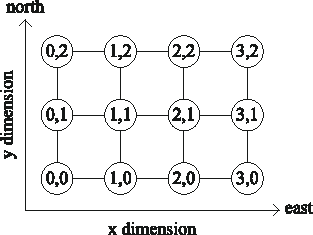
\includegraphics[width=0.5\textwidth]{ZD-fig1}
          \caption{Example of $4 \times 3$ mesh (m=4, n=3).}
        \label{fig:ZD-fig1}
\end{figure}

\subsubsection{Turn Model}
A packet moving toward direction $A$ makes an $AB$ turn if it turns to direction $B$, where $A, B \in {E, W, N, S}$ and $E$ (resp., $W$, $N$, and $S$) refers to direction east (resp., west, north, and south). Note that most routing algorithms prohibit 180-degree turns. Thus, there are eight possible turns, which can form two abstract cycles, clockwise and counter-clockwise abstract cycles. The turn model avoids deadlock by prohibiting one turn in each abstract cycle \cite{glass1992turn}. Since there are four different turns in each abstract cycle, there are totally 16 different combinations to prohibit two turns. Of these 16 combinations, 12 combinations are legal and only three combinations are unique if rotation symmetry is considered. As shown in Figure \ref{fig:ZD-fig2}, they are named as west-first, negative-first, and north-last, resp. 
\begin{figure}[h]
    \centering
        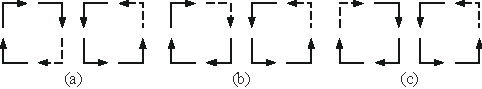
\includegraphics[width=0.85\textwidth]{ZD-fig2}
          \caption{Partially adaptive routing algorithms based on turn model. Forbidden turns are shown as dashed lines. (a) West-first. (b) Negative-first. (c) North-last.}
        \label{fig:ZD-fig2}
\end{figure}


\subsubsection{Odd-Even Turn Model}
The main idea of the odd-even turn model is preventing the formation of rightmost column segments of any circular waiting path \cite{chiu2000odd}. As shown in Figure \ref{fig:ZD-fig3}, there are two kinds of rightmost column, clockwise column and counterclockwise column. The clockwise rightmost column, as shownin Figure \ref{fig:ZD-fig3}(a), consists of an ES turn, an SW turn, and several NS channels. To break the clockwise rightmost column, Chiu \cite{chiu2000odd} proposed to prohibit ES turn in even columns and SW turn in odd columns. To break the counter-clockwise rightmost column, EN and NW turns are forbidden in even and odd columns, resp.

\begin{figure}[h]
    \centering
        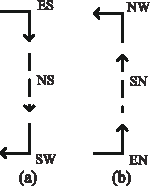
\includegraphics[width=0.3\textwidth]{ZD-fig3}
          \caption{Rightmost column on the waiting path. (a) Clockwise column. (b) Counter-clockwise column.}
        \label{fig:ZD-fig3}
\end{figure}

\subsubsection{Fault Model}
In this paper, we adopt the convex block fault model \cite{boppana1994fault}, in which both node and link faults can be used. For example, a node fault can be modeled by declaring all links incident on it faulty, and a link fault can be used to model partial faults of routers. However, we only consider node fault in this paper for simplicity. Furthermore, we assume that faulty blocks do not share boundaries. If two faulty blocks share a boundary, a bigger faulty block covering the two original ones will be formed. Note that some new fault models, such as the MCC \cite{boppana1994fault} and planar faulty blocks \cite{jiang2008new}, were proposed to reduce the number of fault-free nodes sacrificed by block fault models. Since they are designed for 3-D (or higher dimensional) networks, we omit the detailed discussions in this paper.

\textit{Definition 1:} A convex faulty block is a rectangular contiguous area that consists of danger nodes in 2-D meshes.

\textit{Definition 2:} A node is danger if it is faulty or unsafe.

\textit{Definition 3:} All fault-free nodes are safe initially, and a safe node changes to semi-safe if it has only one danger neighbor. Particularly, if the danger neighbor is in $x$-dimension (resp., $y$-dimension), it changes to semi-safe-x (resp., semisafe-y).

\textit{Definition 4:} A safe or semi-safe node changes to unsafe if: 1) it has two danger neighbors, or 2) it has a danger neighbor in $x$-dimension (resp., $y$-dimension) and a semi-safe-y (resp., semi-safe-x) neighbor.

\textit{Definition 5:} Faulty block’s boundary consists of the safe nodes, which are horizontally, vertically, or diagonally adjacent to this block, and the links between these nodes. Particularly, nodes horizontally or vertically adjacent to the faulty block are called boundary nodes, and those diagonally adjacent are called corner nodes. 

\textit{Definition 6:} The boundary of a faulty block is called a fault ring if the nodes and links form a cycle; otherwise, it is called a fault chain.

\textit{Example 1:} As shown in Figure \ref{fig:ZD-fig4}, an $8 \times 7$ mesh has four faults: (1, 0), (3, 3), (5, 4), and (0, 5). According to Definition 3, nodes (4, 3) and (4, 4) change to semi-safe-x, and nodes (5, 3) and (3, 4) change to semi-safe-y, in the first iteration. According to Definition 4, node (4, 3) changes to unsafe in the second iteration because it has a danger neighbor (3, 3) in x-dimension and a semi-safe-y neighbor (5, 3). Meanwhile, nodes (5, 3), (3, 4), and (4, 4) also change to unsafe according to Definition 4. Faulty blocks are formed in two iterations.

\begin{figure}[h]
    \centering
        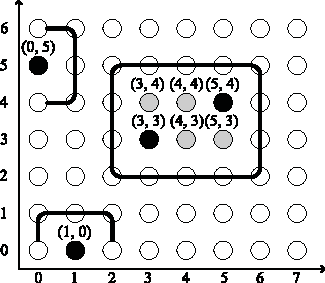
\includegraphics[width=0.6\textwidth]{ZD-fig4}
          \caption{Faulty blocks without shared boundary channels. Dark nodes represent faults and gray nodes indicate unsafet nodes.}
        \label{fig:ZD-fig4}
\end{figure}

It is worthy to note that allowing faulty blocks to share boundaries could further reduce the number of sacrificed fault-free nodes. However, shared boundaries will significantly increase the routing complexity. The discussion about the tradeoffs between the number of sacrificed fault-free nodes and the routing complexity is left as the future work.



\subsection{Fault-Tolerant NoC Architectures}
With device size continuingly scaling down, an increasing likelihood of failure including both transient errors and permanent errors comes to occur within NoC \cite{fan2009godson} \cite{pirretti2004fault}. Both industry designers and academics have paid enormous attention to transient faults \cite{gomez2006routing} \cite{moscibroda2009case} \cite{tsai2012scalable}. In contrast, NoC micro-architecture design for permanent fault tolerant is much less concerned. However, even though permanent fault is not so frequent as transient fault, it is getting pressing nowadays, especially in very large scale ICs \cite{fan2009godson}.

Constantinides et al. \cite{dumitras2003chip} proposed a component-level diagnose and spare-part recon¯guration strategy. With an automatic cluster decomposition algorithm, the proposed method is able to balance area cost and error resilience through replicating and reconfiguring design components in proper granularity. However, this technique is still not a satisfactory minimum overhead design choice. Koibuchi et al \cite{puente2001adaptive}. presented a lightweight fault-tolerant mechanism based on default backup paths (DBP). The method delicately adds DBP instead of complete hardware duplication and consumes much less area overhead. However it takes fault-tolerant design in such a large granularity that the network will soon degrade to a unidirectional ring suffering higher fault rate and thus the network bandwidth degrades dramatically.

Fick et al. \cite{xiang2011efficient} combined ECC (error correcting code), port-swapping, and a crossbar bypass to mitigate wear-out induced hard faults. They exploited inherent redundancy of routers as well as previous bypass method, a kind of resource sparing method similar to DBP, maintaining correct operation and low area overhead. However, it targets the whole port. When only bu®er or link faults appear, the proposed hardware becomes powerless.

Some prior work proposed to serialize transmission channels for defect tolerance \cite{fick2009highly} or protect the link failure \cite{ho2004new} \cite{gomez2006routing}; while in this paper, we take the entire NoC's data path into considerations. And our proposed router microarchitecture design could also tackle the bandwidth mismatch problem between adjacent NoC pipelines. In addition, previous researches such as fault-tolerant routing and network dynamic reconfigurations \cite{dally2004principles} \cite{xiang2011efficient} \cite{fu2011new} \cite{mejia2006segment} are totally orthogonal to the proposed fault-tolerant mechanism, and thus can be combined with the proposed design to further enhance the network reliability.

Fault detection is essential to the proposed fault-tolerant design. In order to precisely know where the fault exists, the built-in self-test (BIST) \cite{wu2003fault} or other on- chip fault detection techniques \cite{flich2008efficient} \cite{rodrigo2010addressing} \cite{feng2012addressing} \cite{li2001loop} can be employed to check the status of the prede¯ned logic blocks, according to which faults will be repaired. Furthermore, some detection error codes (DEC) can be used to find the faults on the control path. There are a lot of available error detection codes like Berger code, parity, Reed Solomon code and other commonly-used CRC.


\section{NoC Fault Tolerance with Topology Reconfiguration}
As technology advances, industry has started to employ multiple cores on a single silicon die in order to improve performance through parallel execution, which has the benefits of power-efficiency and short time-to-market\cite{geer2005chip}. Significant research has been undertaken on tera-scale computing that is able to integrate tens to hundreds of homogeneous processing cores on a single chip to process massive amounts of information in parallel\cite{borkar2007thousand}, \cite{agarwal2007kill}. For example, an 80-core teraflop processor prototype was demonstrated at Intel Developer Forum 2006\cite{computingfew}. Such processors containing a large number of cores are called manycore processors (note the difference from multicore processors that contain a small number of cores). In terms of communication infrastructure, Network-on-Chip (NoC) is generally regarded as the most promising interconnect solution for giga-scale Integrated Circuits (ICs) such as manycore processors \cite{dally2001route,de2008networks}, in which the topology determines the ideal performance of the on-chip network whereas the routing algorithm and the flow control mechanism determine how much of this potential is realized. As a result, Operating System (OS) should understand the topology of NoC-based manycore systems to dispatch and schedule tasks to multiple cores more effectively; while programmers should also be aware of the topology to improve the performance of parallel applications \cite{Microsoft2007numa,stallings2012operating}.

There are many challenges for the architecture design of these NoC-based manycore systems, in which fabrication yield is one of the most serious concerns because an IC’s profitability depends heavily on it \cite{koren1998defect,koren2000should}. With the ever-increasing circuit density, obtaining high fabrication yield solely through improving the manufacturing process is increasingly difficult and will become unaffordable in the near future. For example, as stated in \cite{sperling2007turn}, it would have been lucky to get yield in the range of 10–20 percent for the Cell processor if architectural help is not provided. A more practical solution is therefore to provide defect tolerance capabilities on-chip by incorporating redundant circuits. For example, Memory Built-In-Self-Repair (MBISR) techniques have been widely utilized in the industry and proved to be very effective to keep the high fabrication yield of memory circuits. Such techniques should be extended to other types of VLSI circuits as well \cite{koren1986yield}.

However, tolerating defects in the microprocessor is quite different from tolerating defects in memory because the processor’s internal structure is not as regular as memory cells, and previous attempts in this domain mainly focused on introducing microarchitecture-level redundancy (e.g.,\cite{shivakumar2003exploiting,schuchman2005rescue}). This is appropriate for multicore chips (e.g., a quad-core processor) in order to keep the overhead small. When the number of on-chip cores increases to a point that single core becomes inexpensive when compared to the entire chip (e.g., a 64-core processor), however, it is not necessary to tolerate defective cores at the microarchitecture level. Instead, it is more appropriate to employ core-level redundancy in such case to reduce the complexity associated with microarchitecture-level redundancy.

For NoC-based manycore systems with core-level redundancy, faulty cores are replaced by spare ones placed on-chip. Therefore, it is possible that the topology of the target design is modified and different fabricated chips may have different underlying topologies. This is a big burden for programmers because an optimized program for one topology may not work well for a different one and the programmers are facing various topologies when optimizing their parallel programs.

To address the above problem, the concept of virtual topology is reintroduced from prior network embedding problem in this paper. A virtual topology is isomorphic with the topology of the target design but is a degraded version. From the viewpoint of OS and programmers, they always see a unified virtual topology regardless of the various underlying physical topologies. This eases the dispatching and scheduling tasks for OS and facilitates the optimization of parallel programs. The above issue was briefly discussed in \cite{zhang2007fault}. When compared to \cite{zhang2007fault}, in this paper we re-define the problem by introducing two new metrics, namely Distance Factor (DF) and Congestion Factor (CF), to evaluate the performance of different virtual topologies. We also introduce new algorithms to tackle the problem, and conduct extensive simulation experiments to verify the effectiveness of the proposed solution.

\subsection{NoC Topology Reconfiguration}
\subsubsection{Core-Level Redundancy in Homogeneous Manycore Processors}
As the internal structure is not as regular as memory cells, previous research work on defect tolerance in microprocessors mainly focused on introducing microarchitecture-level redundancy. Redundancy improves yield while at the same time may reduce the chip performance. Researchers thus evaluate the effectiveness of various redundancy mechanisms using performance averaged yield ($Y_{\text{PAV}}$)\cite{shivakumar2003exploiting} or Yield-Adjusted Throughput (YAT) \cite{schuchman2005rescue}. Performance degradation is measured by the relative Instructions Per Cycle (IPC), i.e., the ratio of the reduced IPC to the maximum IPC of the perfect version.

\begin{figure}[t]
    \centering
        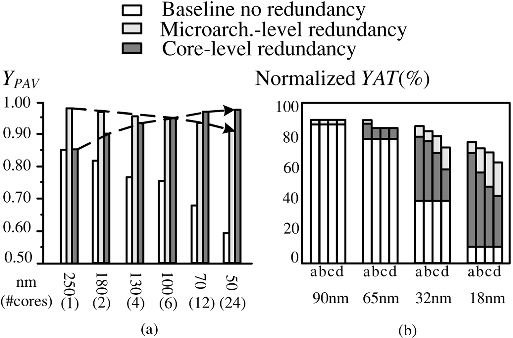
\includegraphics[width=8.5cm]{TR-fig1}
          \caption{ Comparison between microarchitecture- and core-level redundancy.
          (a) comparison redrawn from \cite{shivakumar2003exploiting} with the permission of the author.
          (b) YAT comparison redrawn from \cite{schuchman2005rescue} with the permission of the author.}
             \label{fig1}
\end{figure}

For multicore and manycore processors, the chips themselves naturally have regularity and redundancy as they contain a number of cores. As a result, core-level redundancy could be employed besides microarchitecture-level redundancy. Microarchitecture- and core-level redundancy are named intra- and inter-processor redundancy respectively in \cite{shivakumar2003exploiting}. In the former case, a core can be in any degraded states, but the entire chip is considered bad once the available intra-processor redundancy is exhausted in even one of its cores. In the latter case, a core becomes useless if it contains any faults. However,as long as enough of the remaining cores are functional, the chip is considered to be operational.

Various types of microarchitecture-level redundancies are considered with core-level redundancy by using poisson yield model in \cite{shivakumar2003exploiting}. SPEC2000 and a speech recognition benchmark are chosen to get the IPC reduction. The results are reproduced and shown in Fig.\ref{fig1}(a). The x-axis shows the feature size and the number of cores per chip at each technology. As can be seen in the figure, although there are significant benefits by using microarchitecture-level redundancy when compared to baseline model, $Y_{\text{PAV}}$ drops from 98\% at 250 nm to 91.3\% at 50 nm. Core-level redundancy covers the entire area of the chip and therefore $Y_{\text{PAV }}$ increases uniformly from 85.4\% to 98\%. The yield benefits offered by microarchitecture-level and core-level redundancy crossover at 100 nm.

The authors in \cite{schuchman2005rescue} proposed a novel defect tolerant microarchitecture (namely $Rescue$). Core-level redundancy (called “core sparing” in their work), is used to compare with $Rescue$ by using HotSpot model and negative binomial yield model. IPC reduction is evaluated by simulating 23 benchmark programs from SPEC2000. It also assumes a 20\%(a), 30\%(b), 40\%(c), and 50\%(d) growth of core complexity starting from one core per chip at the 90 nm. The results are redrawn and shown in Fig.\ref{fig1}(b). Similarly, we can observe, as technology advances, YAT becomes increasingly lower without redundancy. At the same time, microarchitecture-level redundancy brings YAT improvement, but at a smaller scale when compared to core-level redundancy in newer technology generation. Microarchitecture-level redundancy shows greater improvement under larger core complexity growth, because the chip has fewer cores and each defective core disables a larger portion of the chip.

From the above analysis, we can conclude that, for manycore chips, because the number of on-chip cores is large and they are fabricated in latest technology, the probability of an embedded core being defective is quite small. Each degraded chip contains a majority of fully functional cores and a small number of defective ones. Therefor, it is not necessary to tolerate defective cores at the microarchitecture-level. Instead, it is more appropriate to employ core-level redundancy in such case to reduce the complexity associated with microarchitecture-level redundancy.

In fact, industry has started to employ core-level redundancy in their products recently. For example, while the Cell processor contains eight Synergistic Processing Elements (SPEs), Sony’s PlayStation 3 video game console considers using only seven of them to increase the manufacturing yield \cite{sperling2007turn}. This approach is also applied in Sun’s UltraSPARC T1 processor \cite{parulkar2002scalable}, \cite{tan2006testing} and Azul’s Vega2 chip \cite{makar2007testing}.

There are two schemes to design homogeneous multicore or manycore chips with core-level redundancy, namely As Many As Available(AMAA) and As Many As Demand(AMAD). The AMAA scheme, adopted in the T1 processor, degrades a chip by disabling faulty cores only. For example, a fabricated quad-core processor can be a full version with 4 functional cores; or it can be degraded to a tri-core, dual-core or single-core processor depending on the number of faulty cores. In AMAD scheme, also denoted as “$N+M$” mechanism in this paper, adopted in the Cell processor ($N=7, M=1$), an -core processor is provided with redundant cores and we always provide customers with operational cores. That is, it is possible that there are fault-free cores left unused in AMAD.

It is preferred to employ the AMAA scheme in multicore to keep the overhead small. However, as the number of on-chip cores increases, the overhead of leaving a few redundant cores on-chip unused is acceptable because a single core is inexpensive compared to the entire chip as discussed above. In addition, with many cores implemented on-chip, we may get various types of degraded chips (with different number of faulty cores) after fabrication and the yield of the demanded-core processor cannot be promised in AMAA scheme. Finally, from a commercial point of view, it may cause some confusion in marketing with many different degraded versions. Therefore, for manycore processors, AMAD scheme is preferred and we mainly focus on this scheme in this paper.

Manycore processors typically use NoC as the communication infrastructure, in which the topology determines the ideal performance whereas the routing algorithm and the flow control mechanism determine how much of this potential is realized. However, in AMAD scheme, as the cores that are fabricated to be defective are not known a priori, when they are replaced by spare cores, the topology of the target design can be different. For example, suppose we want to provide 9-core processors with 3 $\times$ 3 2D mesh topology to customers, as shown in Fig.\ref{fig2}(a). Also, suppose 3 redundant cores (1 column) are provided to improve the yield of these chips as shown in Fig.\ref{fig2}(b). If some cores (no more than 3) are defective, we could still get 9-core processors. However, as shown in Fig.\ref{fig2}(c), if faulty cores are replaced by spare cores, not only the topologies that we get are different from what we expect, but also the topologies of different chips can be distinct. These changed topologies become irregular and would cause performance degradation for manycore processors.

\subsubsection{Topology Impacts on NoC-Based Manycore Systems}

In NoC-based homogeneous manycore systems, the performance of the on-chip communication significantly affects the efficiency of parallel applications. As a result, to minimize the communication overhead among threads or tasks, today’s OS relies on explicit knowledge of the underlying topology \cite{stallings2012operating}. For example in Microsoft Windows Server 2003, a so-called Advanced Configuration and Power Interface (ACPI) circuit is used to pass a description of the physical topology of the system to OS \cite{Microsoft2007numa}. The topology information is stored in Static Resource Affinity Table (SRAT), and is used by Windows when dispatching and scheduling tasks. For example, a representative scheme, namely Gang Scheduling \cite{gupta1991impact}, divides processors into groups, in which processors of the same group have lower communication overhead. Tasks that frequently communicate with each other will be assigned to processors in the same group to minimize communication overhead.

\begin{figure}[t]
    \centering
        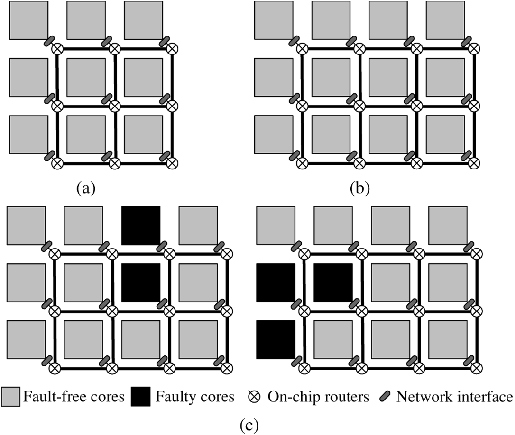
\includegraphics[width=8.5cm]{TR-fig2}
          \caption{ Faulty cores change the topology of target design. (a) What we expect.
          (b) What we implement. (c) What we get.}
             \label{fig2}
\end{figure}

In addition, from the parallel programmers’ perspective, to optimize the performance of the application software, currently they need to know the underlying manycore’s organization \cite{patterson2016computer}. For example, topology information is provided to programmers through API functions in Windows Server 2003. This is the communication-exposed programming for NoC platforms \cite{de2008networks}. Such tailored programs may be not portable to other processors due to different system architectures, such as the number of on-chip cores and their topology.

\subsubsection{Physical Topology and Virtual Topology}
As shown in Fig.\ref{fig2}, faulty cores change the target topology and different chips may have distinct underlying topologies. It would be rather cumbersome for OS and programmers to face various different topologies and optimize them differently. To address this problem, we propose to provide a unified virtual topology regardless of the underlying one. Before introducing the details, we first define $Reference\ Topology$ as the topology of the target design that we expect. For example, the 3 $\times$ 3 2D mesh topology in Fig.\ref{fig2}(a) is the expected reference topology.

For the illustrative “$9+3$” manycore processor shown in Fig.\ref{fig2}(b), suppose the 7th, 10th and 11th cores are defective after fabrication as shown in Fig.\ref{fig3}(a), these cores are considered to be removed out of the chip. The remaining fault-free cores and their interconnections construct a $Physical\ Topology$ as shown in Fig.\ref{fig3}(b). It should be emphasized that once a manycore processor is taped out, its physical topology is determined and cannot be changed during its lifetime. This is fundamentally different from board-level multiprocessor systems, which are much easier to be repaired since the target topology can be maintained by simply replacing the faulty processor with a good one.

\begin{figure}[t]
    \centering
        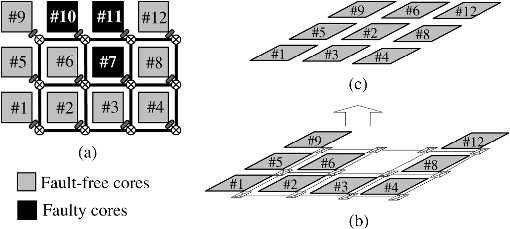
\includegraphics[width=8.5cm]{TR-fig3}
          \caption{ Physical topology and virtual topology. (a) A chip with faulty cores.
          (b) The physical topology. (c) A virtual topology.}
             \label{fig3}
\end{figure}

Based on our AMAD scheme, a 9-core processor can still be provided but with different topology when compared to the reference topology. That is, we can construct a $Virtual\ Topology$ of the chip based on the given physical topology, which is isomorphic with the reference topology. An example is shown in Fig.\ref{fig3}(c), in which we construct a $virtual$ 3 $\times$ 3 2D mesh topology.

With the above configuration, the 3rd, the 5th, the 6th and the 8th cores are four virtual neighbors of the 2nd core. The 3rd core is considered to be below the 2nd core virtually, although it locates at the 2nd core’s right-hand side physically. In addition, while the 5th core is more than one hop away from the 2nd core, they are considered to be adjacent in the above virtual topology.

By using virtual topology, OS and programmers always see a unified topology that is isomorphic with the reference topology, no matter how the underlying cores are connected physically. This greatly simplifies task dispatching and scheduling duties for OS and also facilitates the optimization of parallel programs. In addition, a unified topology that isolates various physical topologies for different chips also significantly eases marketing
process.

A similar idea has been applied in Cray T3E network \cite{scott1996cray}. If some processors fail during the operation of the system, one or more of them may not be physically contiguous. To continue providing applications with a contiguous range of virtual processor numbers, the routing table along with the logical “who am I” registers allows the nodes to be logically renamed, i.e., mapping from physical to virtual number. This kind of “hot swapping” is totally transparent to users. As mentioned above, the failure of nodes and the change of topologies in systems such as Cray T3E are temporary and can be easily recovered because a faulty processor is removed from the system and replaced while OS and user jobs are kept running on the healthy nodes. However, for manycore processors, defects are permanent and physical topologies cannot be recovered. It should be also noted that, depending on the architecture design of manycore processors, there are many ways to implement the mapping from various physical topologies to their corresponding virtual topology. For example, one possible solution is to add a firmware layer below OS to record mapping information which is obtained after fabrication test. This is similar to the CORE\_AVAILABLE\_REG used in UltraSPARC T1 processor \cite{parulkar2002scalable,tan2006testing}. OS and programmers always work on the reference topology while the firmware is responsible for transformation.

\subsection{NoC Topology Virtualization Formulation}
On-chip faulty cores change the topology of the target design and cause performance degradation for parallel applications. To tackle this problem, we use virtual topology to provide a unified interface to OS and programmers, no matter how the underlying cores are connected physically. At the same time, however, as there can be many virtual topologies for a particular physical topology and they may affect applications differently, we should choose the one that results in the best performance.

Since there are a wide range of applications with different characteristics running on the NoC-based manycore systems and they may have different requirements on the construction of virtual topologies, it is difficult to evaluate the impact of virtual topologies on various applications at the chip architecture design stage. As a result, we evaluate the performance of virtual topologies themselves and mainly consider the average latency and throughput of different virtual topologies.

In order to do so, from the viewpoint of the NoC, two evaluation metrics are introduced in this section to model the performance degradation of different virtual topologies when compared to the reference topology, namely Distance Factor (DF) and Congestion Factor (CF). For the sake of simplicity, we assume the communication infrastructure to be fault-free in this research work. This assumption can be justified since the routers and links use much less hardware resources when compared to the cores and are thus less vulnerable to defects \cite{fukushi2005genetic}. Also, it would not cause significant overhead to include fault-tolerant features such as Triple Modular Redundancy (TMR) to protect them.

$Distance\ Factor:$ The zero-load latency $T_{0}$ of a topology can be expressed as \cite{dally2004principles}: $T_{0}=H \times t_{r}+D / v+L / b .$. It is composed of three terms. The router delay is    $H \times t_{r}$ for a network with an average hop count of $H$ and a delay of $t_{r}$  through a single router. The time of flight is$ D / v $ for a network with an average distance of  $D$  and a propagation velocity of  $v$ . The last one is the serialization latency which is the time for a packet of length $L$ to cross a channel with bandwidth $b$.

For a particular physical topology, virtual topologies differ from each other only in the average hop count $H$. When com- pared to reference topology, it is obvious that the average hop count of an irregular virtual topology becomes larger and thus the zero-load latency becomes longer. The distance factor is used to evaluate such degradation, in which $\mathrm{DF}_{n n^{\prime}}$between two nodes $n$ and $ n^{\prime}$ is defined as the physical hops between them $\left(\mathrm{DF}_{n n^{\prime}}=\mathrm{Hops}_{n n^{\prime}}\right)$ and the distance factor of node $n\left(\mathrm{DF}_{n}\right)$ is defined as the average distance factor between node $n$   and all its $k$ virtual neighbors

\begin{figure}[t]
    \centering
        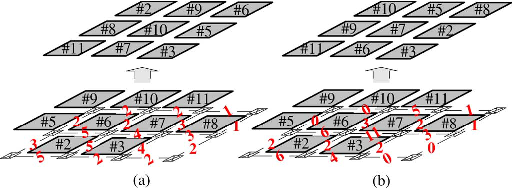
\includegraphics[width=8.5cm]{TR-fig4}
          \caption{ CF comparison between two virtual topologies with the same DF $(\mathrm{DF}=2)$ for a given physical topology. (a) Virtual topology I. (b) Virtual topology II.}
             \label{fig4}
\end{figure}

\begin{equation}
    \mathrm{DF}_{n}=\frac{1}{k} \sum_{n^{\prime}=1}^{k} \mathrm{DF}_{n n^{\prime}}
            \label{eq1}
\end{equation}

Finally, the distance factor of a virtual topology (DF) is defined as the average $\mathrm{DF}_{n}$ of all nodes

\begin{equation}
    \mathrm{DF}=\frac{1}{N} \sum_{n=1}^{N} \mathrm{DF}_{n}
            \label{eq2}
\end{equation}

(There are in total $N$ nodes in the virtual topology.)

The reference topology has the minimum DF as usually virtual neighbors are located next to each other physically. For example, DF is 1 in mesh and torus topologies, which means that each pair of virtual neighbors is exactly one hop away from each other. Larger value of DF means longer communication delay among virtual neighbors.

$Congestion Factor:$ For a given physical topology, it is likely that there are several virtual topologies with the same DF values, as shown in Fig.\ref{fig4}. We therefore use congestion factor to further evaluate the performance of virtual topologies. A virtual topology not only changes the average hop count among cores but also affects the distribution of channel load. Traffic may be- come unbalanced among different links. As the more balanced the channel load, the closer the throughput of the network is to the ideal case \cite{dally2004principles}, a virtual topology that could balance traffic more evenly across all NoC links is preferred.

According to the previous discussion, traffic distribution in NoC-based manycore systems has the property of spatial locality, i.e., communication is more likely to happen between adjacent cores rather than distant ones. We thus only consider the case where a node only communicate with its virtual neighbors. We define the congestion factor of a physical link $l$ (denoted as $\mathrm{CF}_{l}$) as follows: for any nodes $n$ and $ n^{\prime}$ , if they are virtual neighbors, and $l$ is on one of the routing paths between them according to the NoC’s routing mechanism (e.g., XY-routing \cite{de2008networks}), we add $\mathrm{CF}_{l}$    by 1. For the two virtual topologies in Fig.\ref{fig4}, the $\mathrm{CF}_{l}$ values are shown above each physical links. It is clear that traffic in topology I is much balanced than the one in topology II. In topology II, some links are much congested ($\mathrm{CF}_{l}=11$) while some others are barely used ($\mathrm{CF}_{l} = 0$).      .

\begin{figure}[t]
    \centering
        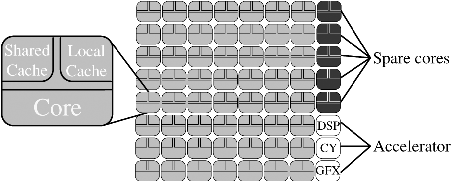
\includegraphics[width=8.5cm]{TR-fig5}
          \caption{ System organization for manycore platform with “$N+M$” scheme.}
             \label{fig5}
\end{figure}

Based on the above observation, we define the congestion factor of a virtual topology (CF) as the standard deviation of $\mathrm{CF}_{l}$ of all links to indicate the traffic distribution

 \begin{equation}
     \mathrm{CF}=\sqrt{\frac{\sum_{l=1}^{L}\left(\mathrm{CF}_{l}-\overline{\mathrm{CF}_{l}}\right)^{2}}{L-1}}
 \end{equation}

 (There are in total $L$ links in the physical topology.)

CF of the reference topology is 0, which means that traffic can be more balanced across the network$\footnote{Please note, congested links are usually revealed around the middle of network even for uniform traffic pattern in practice, CF metric is mainly for comparison purpose and 0 is its ideal upper bound.}$. Greater CF means less even flow distribution. Please note that even though advanced routing algorithms can be introduced to balance channel load, CF can be an auxiliary performance metric to evaluate the raw flow distribution which reflects the quality of a virtual topology. With the above two metrics, the quality of different virtual topologies can be evaluated and compared. DF and CF might be conflicted with each other during optimization, hence we unify them together. The Unified Metric (UM) is defined as

 \begin{equation}
     \mathrm{UM}=w_{\mathrm{DF}} \times \mathrm{DF}+w_{\mathrm{CF}} \times \mathrm{CF}
             \label{eq4}
 \end{equation}

 in which $w_{\mathrm{DF}}$ and   $w_{\mathrm{CF}} $    are the optimization weights designated by users ($w_{\mathrm{DF}} + w_{\mathrm{CF}} =1$).

Reconfiguration from physical to virtual topology is very complex and it depends heavily on the system organizations, such as the reference topology, the on-chip redundancy distribution, etc. In this paper, we mainly focus on mesh and torus topologies, which are the most widely used ones in NoC-based manycore systems. We adopt a representative scalable manycore architecture proposed by Intel as our platform model, which integrates an array of tens to hundreds of streamlined processing cores and accelerators connected by a scalable NoC infrastructure \cite{computingfew}, as shown in Fig.\ref{fig5}. We formulate the topology reconfiguration problem for 2D mesh/torus topology investigated in this paper as follows:

$[Topology\ Reconfiguration\ Problem (TRP)]:$ For an $R \times C$ homogeneous manycore processor with $S$ redundant cores, suppose $D$ cores $(D \leq S)$   are faulty, construct $R \times C$ coordinates as follows:\\

 \begin{figure}[t]
     \centering
         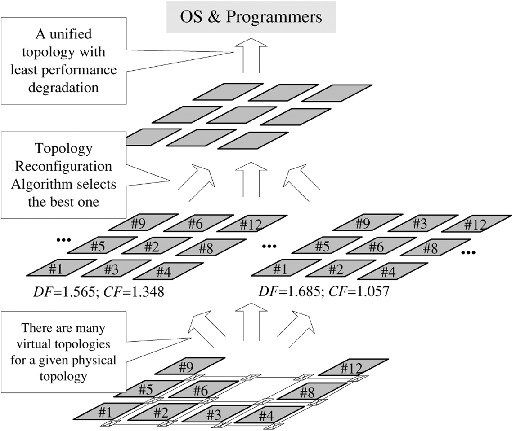
\includegraphics[width=8.5cm]{TR-fig6}
           \caption{Topology reconfiguration.            }
              \label{fig6}
 \end{figure}

 $\left[\begin{array}{cccc}(R-1,0) & (R-1,1) & \cdots & (R-1, C-1) \\ \cdots & \cdots & \cdots & \cdots \\ (1,0) & (1,1) & \cdots & (1, C-1) \\ (0,0) & (0,1) & \cdots & (0, C-1)\end{array}\right]$ \\
     \\
     \\ Distribute these coordinates to $(R \times C+S-D)$  fault-free cores to construct a virtual topology $T_{\text {virtual }}$ , in which nodes with coordinates $(i+1, j),(i-1, j),(i, j+1)$  and  $(i, j-1)$ are four virtual neighbors of node $(i, j)$ , and nodes without being assigned coordinates are left unused, satisfying \\

     \begin{center}
         $\mathrm{UM\ of}\ T_{\text virtual}\ \mathrm{is\ minimized.} $ \\
     \end{center}

Two example virtual topologies for a given physical topology are shown in Fig.\ref{fig6}. The values of DF and CF for these two virtual topologies are also shown in the figure. Clearly, new topology reconfiguration algorithm needs to be developed to select the best candidate topology. Before introducing our pro- posed algorithms, we firstly review prior related work in this area and then give some in-depth analysis of the above TRP problem in the following two sections.

\subsection{NoC Topology Virtualization Optimization}
The objective of TRP in essence is to find a map from virtual locations to physical cores with optimized performance. Considering the configuration shown in Fig.\ref{fig3}, as depicted in Fig.\ref{fig7}, the example virtual topology can be achieved according to the mapping table. For example, virtual location $V$ is mapped to the 2nd physical core. In other words, the 2nd fault-free core is placed in virtual location $V$ in the virtual topology. For the given physical topology in Fig. 7, there are 9! possible virtual topologies with different DF and CF values, because a fault-free core can be placed in any virtual locations.

\begin{figure}[t]
    \centering
        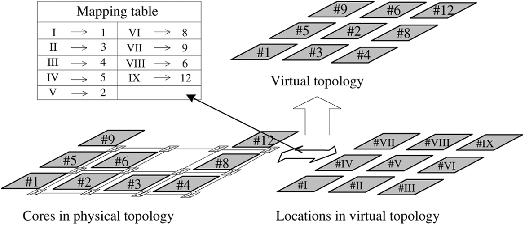
\includegraphics[width=8.5cm]{TR-fig7}
          \caption{ The essence of TRP is to find a map from virtual locations to physical cores.}
             \label{fig7}
\end{figure}

The topology reconfiguration problem can be broken into two related subproblems, to minimize DF and to minimize CF, which we call TRP-I and TRP-II, respectively. In this section, we first recast these two problems from an optimization problem to a decision problem, and then show both of them are essentially instances of known NP-complete problems.

\subsubsection{TRP-I: An Instance of Quadratic Assignment Problem}
According to the above analysis, the decision form of TRP-I can be formulated as follows:

\textbf{[TRP-I]} Virtual locations are numbered $\{1,2 \ldots, n\}$ , while physical cores are numbered $\{1,2 \ldots, m\}, n \leq m$. $d_{k l}$ is the distance (number of $hops$) between physical nodes $k$  and $l$ . $d_{k l}=\infty$ if $k$  or $l$ is defective. Is there a one-to-one function  $f:\{1,2 \ldots, n\} \rightarrow\{1,2, \ldots, m\}$ to construct a virtual topology $T$, such that:$\mathrm{DF}(T) \leq B$ (bound $B \in Z^{+}$).

To ease analysis, suppose the reference topology is torus. Each virtual location $i$ has four neighbors in torus. According to (\ref{eq1}), the distance factor of $i$ can be expressed as $\mathrm{DF}_{i}=(1) /(4) \sum_{j} d_{f(i) f(j)}$ , in which $j$ indicates four virtual neighbors of $i$  and $d_{f(i) f(j)}$    represents the physical distance of node $i$ and its virtual neighbors as mentioned above. The above formulation can be similarly applied for mesh topology, except that the coefficients for different nodes can be 1/2, 1/3, or 1/4, as a virtual node in mesh may have 2, 3, or 4 neighbors based on its position.

From the above, according to (\ref{eq2}) the distance factor of the virtual topology $T$ is

\begin{equation}
    \mathrm{DF}(T)=\frac{1}{4 n} \sum_{i=1}^{n} \sum_{j} d_{f(i) f(j)}
            \label{eq5}
\end{equation}

We now show that TRP-I is essentially an instance of Quadratic Assignment Problem (QAP), which is a well-known NP-complete problem \cite{sahni1976p}. QAP can be formulated as follows \cite{hartmanis1982computers}.

\textbf{[QAP]} Non-negative integer cost: $c_{i j}, 1\leq i, j \leq n$; and distance$d_{k l}, 1 \leq k, l \leq m$ . Is there  a one-to-one  $f:\{1,2 \ldots, n\} \rightarrow\{1,2 \ldots, m\}$  such that:$\sum_{i=1}^{n} \sum_{j=1}^{n} c_{i j} d_{f(i) f(j)} \leq B$.

A QAP instance can be expressed as 
$\left\{\left\langle c_{i j}, d_{k l}, B\right\rangle, c_{i j}, d_{k l}, B \in Z^{+} ; 1 \leq i, j \leq n ; 1 \leq k, l \leq m\right\}$
The famous “backboard wiring” problem \cite{steinberg1961backboard} is a typical application of QAP, which concerns how to place computer components to minimize the total amount of wiring required to connect them.

Considering a QAP instance $\left\{\left\langle c_{i j}, d_{k l}, B\right\rangle\right\}$, let $i$ and $j$ be virtual locations $(1 \leq i, j \leq n)$ in torus, and $d_{k l}$ is the distance between physical nodes $k$ and $l$ as defined in TRP-I. $C_{i j}$ is defined as follows:

$$\left\{
    \begin{array}{ll}
        c_{i j}=1 / 4 n, & \text { if }\ i\ \text { and }\ j\ \text{ are\ virtual\ neighbors }\\
        0, & \text { otherwise.}
    \end{array} \right.
$$ \\

Then the objective of this QAP becomes
\begin{equation}
    \frac{1}{4 n} \sum_{i=1}^{n} \sum_{j} d_{f(i) f(j)} \leq B
    \label{eq6}
\end{equation}

in which $j$ are four virtual neighbors of $i$. According to (\ref{eq5}) and (\ref{eq6}), it is clear that the objective of the above QAP instance becomes to find a mapping function or in other words a virtual topology $(T)$ with distance factor not exceeding $B$. As a result, TRP-I is an instance of the quadratic assignment problem.

\subsubsection{TRP-II: An Instance of Vectorial Quadratic Assignment Problem}
Similarly, the decision form of TRP-II can be formulated as follows. \textbf{[TRP-II]} Virtual locations are numbered $\{1,2 \ldots, n\}$, while physical cores are numbered $\{1,2 \ldots, m\}, n \leq m$. Is there a one-to-one function $f:\{1,2, \ldots, n\} \rightarrow\{1,2 \ldots, m\}$ to construct a virtual topology $T$, such that: $\mathrm{CF}(T) \leq B$(bound $B \in Z^{+}$).

In this subsection, we show that TRP-II is also an instance of quadratic assignment problem, but with a different form. To prove this, we first define a Vectorial Quadratic Assignment Problem (V-QAP) as follows:

\textbf{[V-QAP]} Non-negative integer cost: $c_{i j}, 1 \leq i, j \leq n$; $P$-dimensional non-negative vector $v_{k l}, 1 \leq k, l \leq m$, and bound $B_{V}=\left(A_{1}, A_{2} \ldots, A_{P}\right)$. For two    $P$-dimensional vectors $V_{1}$ and $V_{2}$ is defined as $\left|V_{1}\right| \leq\left|V_{2}\right|$   . Is there a one-to-one function $f:\{1,2 \ldots, n\} \rightarrow\{1,2, \ldots, m\}$ such that:$\sum_{i=1}^{n} \sum_{j=1 \atop j \neq i}^{n} c_{i j} v_{f(i) f(j)} \leq B_{V}$.

An instance of V-QAP can be expressed as $\left\{<c_{i j}, P, v_{k l}, B_{V}>, c_{i j} \in Z^{+}\right.$, $v_{k l}$ and $B_{V}$ are $P$-dimensional non-negative vectors,$1 \leq i, j \leq n, 1 \leq k, l \leq m\}$. It is easy to see that V-QAP is NP-complete because QAP is in fact one-dimensional V-QAP. We now show that TRP-II is an instance of V-QAP. Suppose the reference topology is 2D mesh or torus with $L$ physical links, denoted as  $l_{1}, l_{2}, l_{3} \ldots, l_{1}$. 

$Definition\ 1: Path\ Vector$ $p_{r s}$ is a $L$-dimensional vector $\left(l_{1}, l_{2}, l_{3} \ldots, l_{L}\right)$ . If $l_{x}(1 \leq x \leq L)$ is on one of the paths from physical node $r$ to $s$ according to the NoC’s routing mechanism (e.g., XY-routing), $l_{x}$ in $p_{r s}$ is 1, otherwise $l_{x}$ is 0. A simple example is shown in Fig.\ref{fig8}, in which XY-routing is used. For example, $p_{14}=(1,0,1,0)$ because packets from 1st core to 4th core pass through links  $l_{1}$ and $l_{3}$.

\begin{figure}[t]
    \centering
    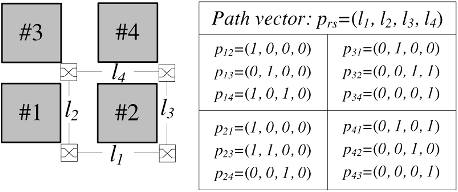
\includegraphics[width=8.5cm]{TR-fig8}
    \caption{Path vector examples.}
    \label{fig8}
\end{figure}

$Definition\ 2: Congestion\ Increment\ Vector$ $v_{r s}$ is defined as $v_{rs}=p_{rs}-I \times d_{rs} / L $, $ d_{rs}$ is the distance between physical node and as defined in TRP-I. $I$ is the $L$-dimensional unit vector.

We now construct a V-QAP instance $\{<\left.c_{i j}, L, v_{r s}, \sqrt{L-1} \times B_{V}>, 1 \leq i, j \leq n, 1 \leq r, s \leq m\right\}$,in which $i$ and $j$ are virtual locations, and $c_{ij}$ is defined as 

$$c_{i j}= \left\{
    \begin{array}{ll}
        1, & \text { if }\ i \text {\ and }\ j \text {\ are\ virtual\ neighbors } \\ 
        0, & \text { otherwise. }
    \end{array} \right. $$

According to the definition of V-QAP, we want to find a one-to-one function $f:\{1,2 \ldots, n\} \rightarrow\{1,2 \ldots, m\}$  such that $\sum_{i=1}^{n} \sum_{j=1 \atop j \neq i}^{n} c_{i j} v_{f(i) f(j)} \leq \sqrt{L-1} \times B_{V}$.

As $c_{i j}$ is 0 if $i$  and $j$ are not virtual neighbors, the objective then becomes $\sum_{i=1}^{n} \sum_{j} v_{f(i) f(j)} \leq \sqrt{L-1} \times B_{V}$, or in another form 

\begin{equation}
    \frac{1}{\sqrt{L-1}}\left|\sum_{i=1}^{n} \sum_{j}\left(p_{f(i) f(j)}-I \times \frac{d_{f(i) f(j)}}{L}\right)\right| \leq\left|B_{V}\right|
    \label{eq7}
\end{equation}

in which $i$ and $j$ are virtual neighbors.

Based on the above definitions of path vector and the congestion factor of a link in Section III, it is not difficult to derive:
$\sum_{i=1}^{n} \sum_{j} p_{f(i) f(j)}=\left(\begin{array}{ll}\mathrm{CF}_{l_{1}}, & \left.\mathrm{CF}_{l_{2}} \ldots \mathrm{CF}_{l_{L}}\right)\end{array}\right.$ and $(1) /(L) \sum_{i=1}^{n} \sum_{j} d_{f(i) f(j)}=\overline{\mathrm{CF}}$. Then, we can conclude from (\ref{eq7}) after substitution:

$(1) /(\sqrt{L-1})\left|\left(\mathrm{CF}_{l_{1}}, \mathrm{CF}_{l_{2}} \ldots \mathrm{CF}_{l_{L}}\right)-I \times \overline{\mathrm{CF}}\right| \leq\left|B_{V}\right|$, i.e., $C F \leq\left|B_{V}\right|$.

It is clear that the above constructed instance of V-QAP is in fact to find a virtual topology($T$) with congestion factor not exceeding $\left|B_{V}\right|$. As a result, we have proved that TRP-II is an instance of V-QAP.

To sum up, we point out that TRP is an instance of the quadratic assignment problem, one of the most complex combinatorial optimization problems. We therefore do not hold much hope for finding an exact polynomial time algorithm for its solution. Efficient and effective heuristics are therefore introduced to solve this problem, as shown in the following section.

On top of the above analysis, an advanced Simulated Annealing (SA) algorithm proposed for QAP is firstly adopted to tackle our TRP. This algorithm, however, is quite time-consuming. We therefore present a fast deterministic greedy algorithm, called Row Rippling and Column Stealing (RRCS). Finally, a $g$SA algorithm is proposed, which outperforms both SA and RRCS algorithms in terms of computing time and the quality of results. It should be noted that we mainly focus on the reconfiguration algorithms for 2D mesh/torus topologies. Other topologies (e.g., butterfly or fat tree topology) may require different optimization algorithms.

\subsubsection{An Adopted Simulated Annealing Algorithm (SA)}
Since we have proved that topology reconfiguration problem is an instance of the quadratic assignment problem, we can adopt previous heuristic approaches for QAP to tackle our TRP. One such approach that has yielded promising results is simulated annealing \cite{misevivcius2003modified,burkard1984thermodynamically,connolly1990improved,bolte1996optimizing}. We adopt one of the most efficient simulated annealing implementations proposed in \cite{misevivcius2003modified} for QAP to tackle TRP in this paper.

Various simulated annealing algorithms generally differ with respect to neighborhood search, annealing schedule and termination criterion. The adopted SA algorithm uses (\ref{eq4}) as the cost function and random virtual topologies as initial solutions. The neighborhood function employed is the widely used “2-exchange”. For example, if the current solution is

\begin{center}
        $\left[\begin{array}{ccc}(1,0) & \text { Faulty } & \text { unused } \\ (0,0) & (0,1) & (1,1)\end{array}\right]$
\end{center}

one of its neighbors by exchanging (1,1) and ‘unused’ is

\begin{center}
        $\left[\begin{array}{ccc}(1,0) & \text { Faulty } & (1,1) \\ (0,0) & (0,1) & \text { Unused }\end{array}\right] .$
\end{center}

The neighboring solutions are searched thoroughly in a fixed order, not randomly. For the above solution, $5 \times(5-1) / 2$ trials are needed to explore all its neighborhood by the sequence (1,0)  $\leftrightarrow$ ‘unused’, $(1,0) \leftrightarrow(0,0), \ldots$ ‘unused’ $\leftrightarrow(0,0),$ ‘unused’ $\leftrightarrow(0,1) \ldots$

The adopted SA algorithm uses the inhomogeneous annealing with oscillation schedules, i.e., temperature is reduced by a very small amount after every trial without any equilibrium test. In addition, temperature is decreased and increased periodically, i.e., reannealing instead of the straightforward annealing, which is the common practice of state-of-the-art simulated annealing algorithms.
The SA algorithm in \cite{misevivcius2003modified} uses an advanced formula to calculate the initial and final temperatures for each iteration, leaving two tuning control parameters, i.e., the initial $\left(\lambda_{1}\right)$ and the final  $\left(\lambda_{2}\right)$ temperature factors, which can be used to control the cooling process effectively.

The algorithm terminates when the current iteration number exceeds $Q$ , or in other words after    $\operatorname{Qn}(n-1) / 2$ trials, in which $n$ is the number of fault-free cores.

\subsubsection{Row Rippling Column Stealing Algorithm (RRCS)}
Simulated annealing is a kind of common technique that can be adopted to all combinatorial optimization problems. However, it does not consider any characteristics of the TRP problem, such as reference topology, system architecture, etc. Moreover, SA is quite time-consuming because it has to explore many random solutions before achieving a satisfactory result. As the configuration time has great impact on the chip cost, SA is not acceptable for large scale manycore systems. As a result,we proposed a fast deterministic greedy algorithm, called Row Rippling and Column Stealing (RRCS) \cite{zhang2007fault}.

\begin{figure}[t]
      \centering
        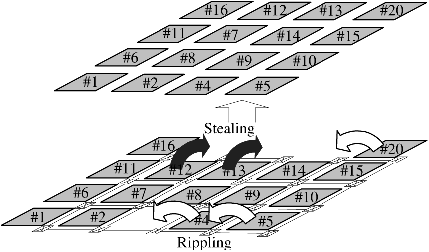
\includegraphics[width=8.5cm]{TR-fig9}
          \caption{An example of RRCS algorithm.}
             \label{fig9}
\end{figure}

\begin{figure}[h]
      \centering
        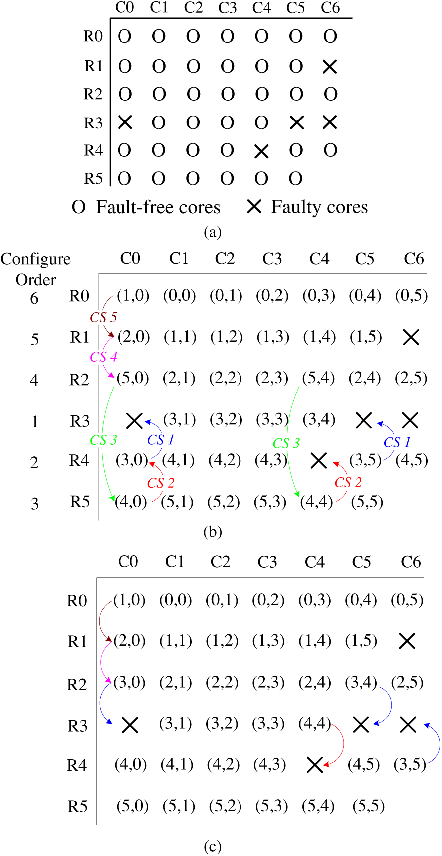
\includegraphics[width=7.5cm]{TR-fig10}
          \caption{Comparison between RRCS and SA. (a) Physical topology. (b) Virtual topology achieved by RRCS $(\mathrm{DF}=1.660 ; \mathrm{CF}=1.428)$. (c) Virtual topology achieved by  $g$SA $(\mathrm{DF}=1.329 ; \mathrm{CF}=0.937)$. }
        \label{fig10}
\end{figure}


RRCS is based on the observation that the performance degradation of a virtual topology is mainly caused by the physical irregularity of the virtual topology compared to the reference topology. Therefore, RRCS algorithm tries to maintain the physical regularity of the virtual topologies in row and in column unit.

To ease illustration, suppose in mesh or torus topology, there are one column of spare cores. If a row contains only one faulty core, i.e., faulty cores are no more than the spare ones in this row, Row Rippling is employed to reconfigure the row, in which a faulty core is replaced by its neighbor and the virtual position of the core used to replace the faulty one is transferred to the next neighboring core. This process continues until the spare one is used to replace the last element in the row. When a row contains more than one faulty cores, i.e., faulty cores are more than the spare ones in this row, the rightmost faulty core is replaced using rippling. The other faulty elements within the row, however, are replaced with the elements immediately beneath them. In other words, we “steal” a fault-free core from another row within the same column. This stolen core should be considered faulty when the row containing it is reconfigured. An example of using RRCS in a “ $16+4$ ” processor with 4 $\times$ 4 mesh reference topology and one column redundancy is depicted in Fig. 9. To configure the uppermost row, which contains 3 faulty cores, we steal the 12th and the 13th fault-free cores for the left two fault cores; while the rightmost one is rippling to the 20th core. Only Row Rippling is used to configure the lowermost row as it contains one faulty core. The achieved virtual topology is shown above the physical topology.

In the above discussion, we provide a column of redundant cores as an example. In practice, the number of redundant cores, i.e.,$M$ , for an $N$-core processor should be carefully determined by the designers in advance (e.g., using the analysis framework in \cite{pan2007framework}), and may be different from the column size. This however does not affect the working mechanism of the proposed RRCS algorithm as it only needs to compare the number of faulty cores   $N_{f}$  and spare cores on each row. We are able to generate an effective virtual topology as long as the number of faulty cores is less than $M$. In the worst case, i.e., all available cores in both the same row and the same column are exhausted, we simply choose a nearest core to replace the faulty one.

\subsubsection{RRCS-Guided Simulated Annealing Algorithm ($g$SA)}
RRCS is very fast when compared to SA algorithm, but it does not directly consider DF or CF metrics during the optimization process. Moreover, RRCS may cause serious chain column stealing operations for certain physical topologies and result in undesirable virtual topologies.

For example, consider a physical topology with 6 $\times$ 6 2D mesh reference topology and 5 spare cores located on the righthand side and 5 faulty cores, as shown in Fig.\ref{fig10}(a). The virtual topology achieved by RRCS is shown in Fig.\ref{fig10}(b), in which the coordinates indicates the virtual locations for the corresponding cores. Reconfiguration begins from row R3, causing two stealing operations, i.e., the two CS1 from row R4. R4 then does not have enough available cores and has to steal another two cores, i.e., CS2 from row R5. The process continues until the last row R0 is configured. Note that CS3 borrows relatively distant cores to configure faulty cores in row R5. These chain column stealing operations will generate an undesirable virtual topology.


At the same time, RRCS is very efficient, and it can arrange most part of the virtual topology in a good shape. We find that by applying several 2-exchange operations on top of the topologies achieved by RRCS, the quality of the results can be greatly improved. As a result, we propose to combine the algorithms of RRCS and SA together. We use RRCS to quickly generate a good initial solution point, and then apply the adopted SA algorithm on top of it to explore its 2-exchange neighboring solutions. We call this strategy RRCS-guided Simulated Annealing technique ($g$SA).

We use $g$SA $\left(w_{\mathrm{DF}}=0.9, w_{\mathrm{CF}}=0.1\right)$ and RRCS working on 100 random physical topologies in 6 $\times$ 6 2D mesh with 5 spare and 5 randomly distributed faulty cores and 8 $\times$ 8 2D mesh with 8 spare and 8 random faulty cores respectively. The DF and CF improvement of $g$SA over RRCS are reordered from small to large and are shown in Fig.\ref{fig11}. For the DF metric in 6 $\times$ 6 array, RRCS generates the same results as $g$SA for the first 28 physical topologies, i.e., no improvement, while for the other 72 cases, $g$SA has different levels of improvement. When the network size increases to 8 $\times$ 8, $g$SA achieves greater improvement than in 6 $\times$ 6 for 80\% cases. CF metric is similar. We can conclude that RRCS is efficient since for around 20\%–35\% cases, it generates results as good as $g$SA. However, for many circumstances due to chain column stealing operations, RRCS has very poor performance, and $g$SA can improve over RRCS greatly, especially for larger network size.

\begin{figure}[h]
      \centering
        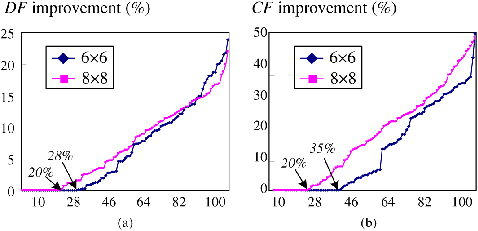
\includegraphics[width=8.5cm]{TR-fig11}
          \caption{$g$SA improvement over RRCS for different network size. (a) DF improvement. (b) CF improvement.}
        \label{fig11}
\end{figure}

We then use SA algorithm with different parameters working on the above 100 physical topologies in 6 $\times$ 6 and 8 $\times$ 8 mesh. The initial and final temperature factors  $\lambda_{1}$   and $\lambda_{2}$  are tuned and set to be 0.5 and 0.05 respectively. We choose 50 and 100 random solutions, i.e., SA-50 and SA-100 with different iteration numbers, i.e., $Q=10$ and $Q=20 \cdot w_{\mathrm{DF}} $  and $w_{\mathrm{CF}}$ are set to be 0.9 and 0.1 respectively. The averaged results are shown in Table \ref{tab:gSA-Improve}. It can be seen that, $g$SA outperforms SA in all cases with very little computational time. With more random solutions and more iteration numbers, SA improves a little but with great computing time overhead. This is because the quality of random initial solutions used by SA are much worse than RRCS, which is able to focus on a good solution point very fast.

\begin{table}
    \caption{gSA Improvement Over SA for Different Network Size}
    \begin{tabular}{c|ccc}
        \hline
         & \multicolumn{3}{c}{$6 \times 6$ 2D mesh with 5 spare and 5 fault cores} \\ \hline
         & SA-50 (Q=10) & SA-100 (Q=20)  & gSA  \\
 Time(s) & 177.4        &  484.7         &  2.2   \\
 DF      & 1.538        &  1.483         &  1.319 \\
 CF      & 1.396        &  1.312         &  0.977 \\ \hline
         & \multicolumn{3}{c}{$8 \times 8$ 2D mesh with 8 spare and 8 fault cores } \\ \hline
         & SA-50 (Q=10) & SA-100(Q=20)   & gSA  \\
 Time(s) & 484.4        & 3477.8         & 8.9    \\
 DF      & 1.782        & 1.473          & 1.296  \\
 CF      & 1.615        & 1.288          & 0.908  \\ \hline
    \end{tabular}
    \label{tab:gSA-Improve}
\end{table}

\subsection{Experiment Result Analysis}
\subsubsection{Experimental Setup}
We have implemented a manycore NoC simulation platform composed of classic pipelined virtual channel routers and cores which generate synthetic workload. The router pipeline has four stages, i.e., routing computation, virtual-channel allocation, switch allocation and switch traversal, in which each stage takes one clock cycle. Since we want to evaluate the performance of virtual topologies, other parameters should remain unchanged. In our experiments, each physical link has 8 virtual channels, and each virtual channel has 8 flit buffers. Credit-based flow control is used for buffer management. To reveal the performance of topologies themselves, the simple dimension-order routing is used which has the minimum impact on traffic distributions.

As execution-driven workload makes it difficult to isolate bottlenecks in the network design \cite{dally2004principles} and we concern more about the network performance, we use synthetic workload instead of execution-driven workload. Each core in our manycore NoC simulation platform is actually a traffic generator. As virtual topologies are constructed based on the spatial locality of communication, we adopt the neighboring traffic pattern in our experiments, in which a core only exchanges information with its neighbors. It is important to point out that the traffic patterns are applied to virtual topologies, not to physical topologies. That is, 1-hop communication between virtual neighbors may involve multiple physical hops.

Virtual topologies generated by reconfiguration algorithms are in XML format to be read by the simulation platform. Each core will then be assigned a name “$c_{-} v t x_{-} v t y_{-} p h x_{-} p h x$”, in which $(v t x, v t y)$  and $(phx, phy)$ are its virtual and physical coordinates. Each time a core sends a packet, it reads its virtual location, looks up the mapping table stored in the simulator to find the physical locations of its virtual neighbors and then encapsulates in the packets as the destination address.

\subsubsection{Experiment I}
In this experiment, we show how predictive of DF and CF metrics to real performance measurements. DF is the average hop count between virtual neighbors and thus should reflect the average delay and throughput of the network. While CF indicates traffic distribution across all the physical channels. We use SA-1 (1 random initial solution), RRCS and $g$SA $\left(w_{\mathrm{DF}}=0.9, w_{\mathrm{CF}}=0.1\right)$  to work on 100 different physical topologies in 8 $\times$ 8 2D mesh with 8 spare cores and 8 randomly distributed faulty cores on-chip. We use SA-1 to keep the computational time comparable to $g$SA. We choose the physical topology on which $g$SA achieves the greatest improvement over SA-1 and RRCS in this experiment. The obtained DF and CF values are shown in Fig.\ref{fig12}.

\begin{figure}[h]
      \centering
        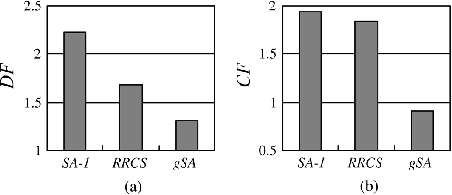
\includegraphics[width=8.5cm]{TR-fig12}
          \caption{ Comparison between SA-1, RRCS and SA. (a) DF comparison. (b) CF comparison.}
        \label{fig12}
\end{figure}


Next, we import virtual topologies generated by these three algorithms into our manycore NoC platform to get the simulation performance measurements, i.e., average delay, throughput and average occupied time of all channels as shown in Fig.\ref{fig13}. 

Average delay is the time required for a packet to traverse the network from source to destination. It can be observed from Fig.\ref{fig13}(a), the latency of virtual topologies achieved by SA-1, RRCS and $g$SA are almost the same under light traffic load. When the network saturates, it is clear that the delayof $g$SA is better than RRCS, and RRCS is better than SA-1. Network throughput is the packets delivering rate for a particular traffic pattern. Fig.\ref{fig13}(b) shows the throughput of saturation of the three algorithms. It is clear that the throughput of $g$SA is higher than RRCS, while RRCS is higher than SA-1. Compared with Fig.\ref{fig12}(a), we show the effectiveness for DF as performance metrics.

Fig.\ref{fig13}(c) shows the percentage of occupied time of all physical channels. More occupied time implies that more traffic passing through that channel. We reorder these values from small to large for easy comparison. It can be observed that the curve for $g$SA has the smallest slope, which means the differences between all channels are small, i.e., the traffic is more evenly distributed. RRCS is more steep than $g$SA, and SA-1 is more steep than RRCS. Compared with Fig.\ref{fig12}(b), we show that the CF metric reflects real performance measurement.

\begin{figure}[h]
      \centering
        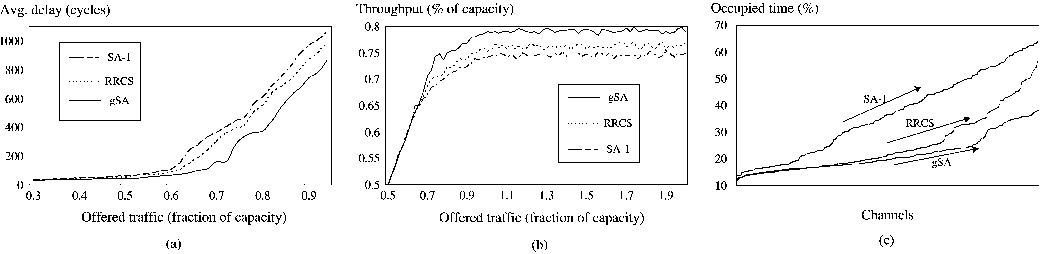
\includegraphics[width=12cm]{TR-fig13}
        \caption{ Simulation measurements comparison between SA-1, RRCS and $g$SA. (a) Average delay. (b) Throughput. (c) Traffic distribution.}
        \label{fig13}
\end{figure}

From the above we can conclude that, $g$SA has better performance than RRCS and SA-1, not only in terms of DF and CF metrics but also in real performance measurements, i.e., latency, throughput and traffic distribution. In addition, the effectiveness of DF and CF as evaluation metrics is proved with this experiment.

\subsubsection{Experiment II}

In this experiment, we evaluate the effectiveness of the proposed  $g$SA algorithm with the scale of network size. We use the 8 $\times$ 8 2D mesh topology with 8 spare cores and 8 randomly distributed faulty cores. We choose another larger configuration with 10 $\times$ 10 2D mesh reference topology, 12 spare cores and 12 random faulty cores for proportional scaling. We work on 100 random physical topologies in 8 $\times$ 8 and 10 $\times$ 10 respectively. The average improvement of $g$SA over RRCS for DF metric is 6.828\% in 8 8 while 9.737\% in 10 $\times$ 10 configurations. Regarding the CF metric, the improvement is 18.935\% in 8 $\times$ 8 and 20.983\% in 10 $\times$ 10 respectively. That means when network becomes larger, $g$SA achieves much better improvement over RRCS.


The average delay, throughput and traffic distribution are shown in Fig.\ref{fig14}. It is clear that $g$SA improves over RRCS for both network sizes. For smaller network size, i.e., 8 $\times$ 8, the averaged delay, throughput and traffic distribution of virtual topologies achieved by RRCS are much closer to that of $g$SA. For larger network size, i.e., 10 $\times$ 10, $g$SA achieves much better improvement in all measurements. Thus we can conclude that, firstly, when network size scales, $g$SA achieves better improvement; secondly, we further validate the effectiveness of DF and CF because the level of improvement for these two metrics and real performance measurements are similar.

\begin{figure}[h]
      \centering
        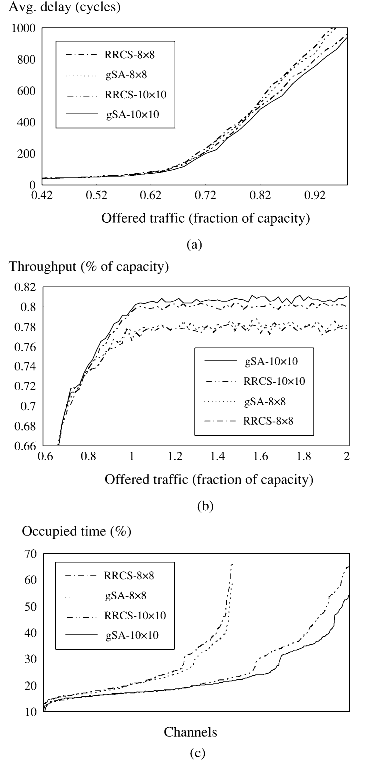
\includegraphics[width=12cm]{TR-fig14}
          \caption{ Comparison between RRCS and $g$SA for different network size. (a) Average delay. (b) Throughput. (c) Traffic distribution.}
        \label{fig14}
\end{figure}


\subsubsection{Experiment III}

In this experiment, we evaluate the impact of different number of faulty cores and spare cores on $g$SA algorithm.

Firstly, we use 8 $\times$ 8 2D mesh with one column spare cores. We vary the number of faulty cores from 2 to 8 (i.e., D2, D4, D6 and D8). Faulty cores are randomly distributed, leading to various physical topologies. Results are averaged and shown in the first two figures in Fig.\ref{fig15}.

It is clear that when the number of defective cores increases, the performance of virtual topologies achieved by $g$SA slightly becomes worse in terms of both DF and CF. This is expected because the increase of faulty cores limits the solution space of the proposed algorithm.

Next, we assume there are always 2 randomly distributed faulty cores in 8 $\times$ 8 2D mesh and we vary the number of spare cores from 2 to 10 (i.e., S2, S4, S6, S8 and S10). As expected, the increase of spare cores also increases the solution space of the $g$SA algorithm, and both DF and CF slightly becomes better. However, when the number of spare cores is increased from 8 to 10, we find that DF almost remains the same while CF becomes much worse as in Fig.\ref{fig15}. This is because there are many cores and channels left unused on-chip, traffic distribution becomes much uneven. Therefore, we can conclude employing more-than-necessary number of spare cores does not facilitate to boost the NoC-based manycore systems’ performance much after reconfiguration.

\begin{figure}[h]
      \centering
        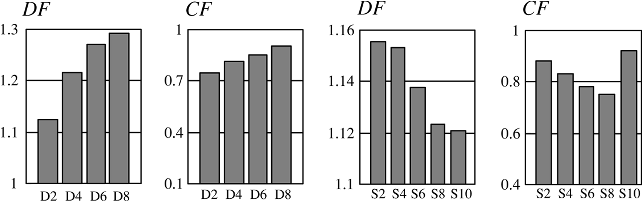
\includegraphics[width=8.5cm]{TR-fig15}
        \caption{ The impact of different number of faulty cores and spare cores on $g$SA algorithm.}
        \label{fig15}
\end{figure}


Effective defect tolerance techniques are essential to improve the yield of homogeneous manycore processors. In this paper, we propose to employ core-level redundancy with AMAD scheme to address this issue. As defective cores change the topology of the target design, programmers may face various different topologies when optimizing their parallel programs. This is a big burden and may also cause confusion in marketing. We propose to address the above problem by providing a unified topology that is isomorphic with the target reference topology regardless of the various possible underlying physical topologies. We borrow the concept of virtual topology from network embedding problem and we propose two metrics to evaluate the performance of different virtual topologies. An effective heuristic, namely Row Rippling Column Stealing-guided Simulated Annealing algorithm is then presented to solve the topology reconfiguration problem. The proposed algorithm is evaluated on various topologies in a NoC-based manycore simulation platform. Experimental results not only show the effectiveness of the proposed $g$SA algorithm, but also show the effectiveness of the two evaluation metrics used in our algorithms, i.e., DF and CF. In our future work, we plan to investigate the topology reconfiguration problems for topologies other than mesh and torus (e.g., butterfly topology).

\subsection{Discussion}
To be added.

\section{NoC Fault Tolerance with Routing}
Fault-tolerant routing is usually used to provide reliable on-chip communication for many-core processors. This paper focuses on a special class of algorithms that do not use virtual channels. One of the major challenges is to keep the network deadlock free in the presence of faults, especially those locating on network edges. State-of-the-art solutions address this problem by either disabling all nodes of the faulty network edges or including all faults into one faulty block. Therefore, a large number of fault-free nodes will be sacrificed. To address this problem, the proposed ZoneDefense routing not only includes faults into convex faulty blocks but also spreads the faulty blocks’ position information in corresponding columns. The nodes, which know the position of faulty blocks, form the defense zones. Therefore, packets can find the faulty blocks and route around them in advance. Exploiting the defense zones, the proposed ZoneDefense routing could tolerate many more faults with significantly reduced sacrificed fault-free nodes compared with the state-of-the-art algorithms. Furthermore, the ZoneDefense routing does not degrade the network performance in the absence of faults, and could get similar performance as its counterparts in the presence of faults.

\subsection{Challenges of Fault-Tolerant NoC Routing}
MANY-CORE processors usually utilize network-on-chip (NoC) to provide on-chip communication \cite{dally2004principles}. 2-D mesh topology is widely adopted since its planar structure facilitates the IC manufacturing. For example, TILE64 \cite{bell2008tile64} and Godson-T \cite{fan2009godson} processors select an 8 × 8 mesh, and Intel Tera-scale prototype processor adopts an 8 × 10 mesh \cite{vangal200880}. The performance of NoC depends heavily on the efficiency of routing algorithm, which is either deterministic or adaptive. Most many-core processors use deterministic routing, such as the X-Y routing, since it facilitates the design of efficient routers \cite{bell2008tile64} \cite{fan2009godson} \cite{vangal200880}. Unfortunately, X-Y routing is not fault-tolerant.

Faults can appear in cores, routers, and other components. Failed cores can be tolerated by redundancy \cite{zhang2009topology}, while failed routers are usually handled by fault-tolerant routing. One of the major challenges of designing fault-tolerant routing is to keep the network deadlock free. The wormhole switching technique and the absence of virtual channels make this problem more challenging. In addition, many-core processors usually use virtual networks to avoid protocol deadlock, where each virtual network is usually assigned with a separate virtual channel. Thus, no virtual channel could be used by the routing algorithm to avoid routing deadlock. From the routing algorithms’ point of view, this kind of NoC is same with that does not have virtual channels.

In NoCs without virtual channels, turn models are usually used to avoid deadlock \cite{glass1992turn} \cite{chiu2000odd} \cite{fu2011abacus}. Chiu \cite{chiu2000odd} has proved that a network is deadlock free if all rightmost columns are removed from the network. However, without rightmost columns, it is difficult to tolerate faults locating on the left network edge \cite{glass1993fault} \cite{wu2003fault} \cite{zhang2008reconfigurable}.

To address this problem, Glass and Ni \cite{glass1993fault}, Wu \cite{wu2003fault}, and Zhang et al. \cite{zhang2008reconfigurable} have proposed their solutions. These solutions either tolerate only one fault \cite{glass1993fault} or disable a large number of fault-free nodes \cite{wu2003fault}, \cite{zhang2008reconfigurable}. One common feature of them is that packets do not know the faults until they are blocked. In our opinion, this is the major reason that causes the difficulties to keep the network deadlock free. Because packets should make a turn to route around faults. However, these turns are usually unexpected and make it difficult to
avoid deadlock.

To address this problem, we propose to include faults into defense zones with which packets could find faults in advance. Based on the defense zones, we propose the ZoneDefense routing that can significantly improve the state-of-theart routing algorithms \cite{glass1993fault} \cite{wu2003fault} \cite{zhang2008reconfigurable}in the following three aspects: 1) the number of sacrificed fault-free nodes, 2) the network reconfiguration time, and 3) the coverage of fault distributions.

\subsection{Defense Zones}
According to \cite{chiu2000odd}, a network is deadlock free if all rightmost columns are removed. As shown in Figure \ref{fig:ZD-fig3}, ES, SW, EN, and NW turns are necessary to form rightmost columns. To distinguish them from others, they are called unexpected turns. Unfortunately, unexpected turns may be introduced if a packet hits the boundary of a faulty block. To avoid unexpected turns, we introduce the defense zones, so that packets could find the faulty block and route around it in advance.

The formation of defense zones is triggered by the detection of faults using such as build-in self-test techniques \cite{li2001loop}. In this paper, we utilize the dynamic fault model, but assume that no new fault occurs during a routing process like \cite{wu2003fault}. However, in practice, faults may occur at any time. To support dynamic faults, one can exploit more reliable flow control techniques, such as APCS \cite{gaughan1996distributed} and the one proposed in \cite{dao1999dynamically}. These techniques are orthogonal with the proposed ZoneDefense routing, so we omit the detailed descriptions. Besides, faulty nodes are assumed to be nonmalicious, i.e., they do not send and receive packets.


Once a fault is detected, the formation of defense zones is logically divided into two steps:
1) construct faulty blocks with fault chains, and identify reference nodes in fault chains if necessary;
2) spread the position of faulty blocks in columns wherein they reside if necessary.


\textbf{\textit{A. Step 1: Forming Faulty Blocks and Identifying Reference
Nodes}}

We have shown the way to form convex faulty blocks in Section II-D. These faulty blocks can be categorized into nine classes based on the types of network edges they touch as shown in Figure \ref{fig:ZD-fig5}. To route around faulty blocks, we utilize fault chains to encapsulate them. If a faulty block touches any one network edge, its boundary naturally forms a chain. Otherwise, we intentionally break the boundary at its northeast corner by forbidding the ES and NW turns as shown in Figure \ref{fig:ZD-fig5}(e).

\begin{figure}[h]
    \centering
        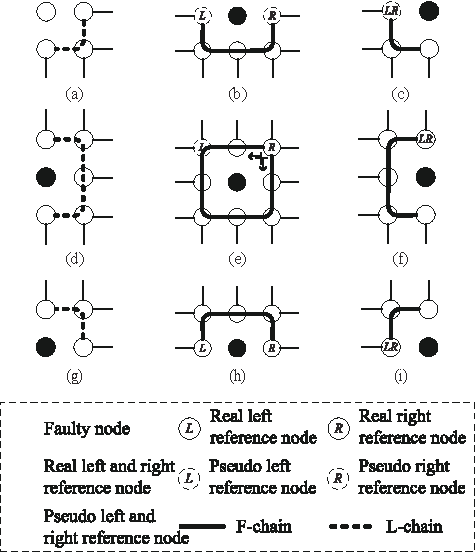
\includegraphics[width=0.7\textwidth]{ZD-fig5}
          \caption{Types of faulty blocks. (a) FB-1. (2)FB-2. (c)FB-3. (d)FB-4. (e)FB-5. (f)FB-6. (g)FB-7. (h)FB-8. (i)FB-9.}
        \label{fig:ZD-fig5}
\end{figure}


The fault chain is called a $l$-chain if the type of faulty block is FB-1, FB-4, or FB-7; otherwise, it is called a $f$-chain. For a $l$-chain, at least one of its two end points touches the left network edge. It is used to notify that there is no route on the west side of the faulty blocks. For $f$-chains, two reference nodes, left ($L$) and right ($R$) reference nodes, should be considered to make correct routing decisions. Furthermore, reference nodes could be real or pseudo. As shown in Figure \ref{fig:ZD-fig5}, left reference nodes are labeled $L$, and right reference nodes are labeled $R$. Real reference nodes are shown as solid circles, and pseudo reference nodes are shown as dashed circles. In fact, the proposed ZoneDefense routing only cares about the height (or the coordinate in $y$-dimension) of reference nodes. As for the real reference node, its height is propagated along the chain. As for pseudo reference node, the number of rows of the mesh is propagated.

The reference nodes are used to separate packets into two classes: the destination is {lower, not lower} than the reference node. This kind of information will be used by the ZoneDefense routing to route around faulty blocks without introducing forbidden turns. More specifically, left and right reference nodes are used to direct westward and eastward packets, resp. The pseudo reference nodes are used to indicate that all destinations are lower than the reference node as shown in Figure \ref{fig:ZD-fig5}(b) and (c). As shown in Figure \ref{fig:ZD-fig5}(e), the left reference node of FB-5 faulty blocks is also pseudo. Thus, all westward packets will be treated as if their destinations are lower than the left reference node, and routed along the clockwise direction without introducing the forbidden NW turn at the northeast corner. Since we only care about the height of reference nodes, the real reference node could be any node in the same raw. For example, the left and right reference nodes of FB-6 faulty blocks, as shown in Figure \ref{fig:ZD-fig5}(f), could also be the northwest corner.

\textbf\textit{B. Step 2: Forming Defense Zones}

To avoid vertically hitting a faulty block’s boundary, nodes above and below it should be notified with the position information of this block. To store that information, two registers are required, \textit{ceiling} and \textit{floor}, as shown in Figure \ref{fig:ZD-fig6}. In the rest of this section, we will discuss the two rules that are used to update the ceiling and floor registers.
\begin{figure}[h]
    \centering
        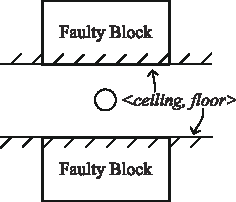
\includegraphics[width=0.4\textwidth]{ZD-fig6}
          \caption{\textit{Celing} and \textit{floor}}
        \label{fig:ZD-fig6}
\end{figure}


\textit{Ceiling Rule:} the \textit{ceiling} register of all safe nodes is initialized to $n$, where $n$ is the number of rows of the $m \times n$ mesh. This means that there are no faulty blocks above that node. The value of \textit{ceiling}.

\begin{enumerate}[1)]
    \item Changes to $C_{y}$, where $C_{y}$ is the $y$-coordinate of current node, if it is the south boundary node of FB-5 and FB-6 faulty blocks;

    \item Otherwise, changes to $N_{y}$, where $N_{y}$ is the $y$-coordinate of the north neighbor, if the north neighbor is the northwest corner of FB-8 faulty blocks or the northeast corner of FB-5 faulty blocks;

    \item Otherwise, changes to \textit{ceiling\_n}, where \textit{ceiling\_n} is the value of ceiling register of the north neighbor, if the north neighbor is NOT danger.
\end{enumerate}

\textit{Floor Rule:} the \textit{floor} register of all safe nodes is initialized to 0. The value of \textit{floor:}

\begin{enumerate}[1)]
    \item Changes to $C_{y}$, where $C_{y}$ is the $y$-coordinate of current node, if it is the north boundary node of FB-5 and FB-6 faulty blocks;
    \item Otherwise, changes to $S_{y}$, where $S_{y}$ is the $y$-coordinate of the south neighbor, if the south neighbor is the southwest corner of FB-2 and FB-5 faulty blocks or the northeast corner of FB-5 faulty blocks;
    \item Otherwise, changes to \textit{floor\_s}, where \textit{floor\_s} is the value of floor register of the south neighbor, if the south neighbor is NOT danger.
\end{enumerate}

Based on the above two rules, the position information of all kinds of faulty blocks, which can introduce unexpected turns, are propagated to corresponding nodes. Thus, packets could utilize the position information to avoid introducing deadlock. For example, if a packet vertically hits the south boundary of FB-5 or FB-6 faulty blocks, an NW turn will be introduced. According to the first \textit{ceiling rule}, south boundary nodes of FB-5 and FB-6 faulty blocks update their ceiling registers using their own y-coordinates. The value of ceiling is further propagated to south neighbors according to the third \textit{ceiling rule}. By comparing the destination’s y-coordinate with the ceiling, we can know that whether routing a packet to north will introduce an NW turn. If the answer is yes, we can route packet to west instead of north to avoid the unexpected NW turn. In the next section, we will discuss how does the proposed ZoneDefense routing algorithm route packets based on defense zones.

\subsection{ZoneDefense Routing Algorithms}
ZoneDefense routing (see Algorithm \ref{alg:routing1}) routes packets according to the type of node currently the header flit resides in. If the header flit arrives at the destination, the packet is consumed. Otherwise, the header flit is first routed by the Default-Routing. After that, if the current node is on a fault chain, the output is redirected by two routing subfunctions: LChain-Routing and FChain-Routing.

\begin{algorithm}
    \caption{ZoneDefense-Routing}
    \label{alg:routing1}
    \KwData{$C:$ current node; $D:$ destination node.}
    \KwResult{$output$}
    \uIf{C=D}{
        Consume the packet\;
    }
    \Else{
        $output$=Default-Routing()\;
        \uIf{Current node is shared by a $l$-chain and a $f$-chain}{
            \uIf{$output=west$}{
                $output$=LChain-Routing()\;
            }
            \Else{
                $output$=FChain-Routing()\;
            }
        }
        \uElseIf{Current node is on a $l$-chain}{
            $output$ = LChain-Routing()\;
        }
        \ElseIf{Current node is on a $f$-chain}{
            $output$=FChain-Routing()\;
        }
    }
\end{algorithm}

According to the Default-Routing (see Algorithm \ref{alg:routing2}), the packet is routed to west if the destination is on the west to the current node. Otherwise, the Default-Routing tries to route packets following the $Y-X$ routing rules. However, if the destination is higher than \textit{ceiling} or lower than \textit{floor}, the packet should be first misrouted to west to avoid vertically hitting the faulty block boundaries. Otherwise, an NW or SW turn will be made.

\begin{algorithm}
    \caption{Default-Routing}
    \label{alg:routing2}
    \KwData{$C:$ Current node; $D:$ destination node.}
    \KwResult{$output$}
    \uIf{$C_{x}>D_{x}$}{
        $output=west$\;
    }
    \uElseIf{$C_{x} \neq 0$ and ($D_{y} > ceiling$ or $D_{y} < floor$)}{
        $output=west$\;
    }
    \uElseIf{$C_{y}<D_{y}$}{
        $output=north$\;
    }
    \uElseIf{$C_{y}>D_{y}$}{
        $output=south$\;
    }
    \Else{
        $output=east$\;
    }
\end{algorithm}

If the current node is on a fault chain, the routing path assigned by Default-Routing may be blocked by faults. Thus, the output port should be redirected. More specifically, when the current node is the corner shared by a $l$-chain and a $f$-chain, the LChain-Routing (see Algorithm \ref{alg:routing3}) will be used if the Default-Routing selects the west output. Otherwise, the FChain-Routing (see Algorithm \ref{alg:routing4}) will be used. If the current node is not shared by fault chains or shared by two $f$-chains, the routing subfunction is selected based on the type of fault chain.

\begin{algorithm}
    \caption{LChain-Routing}
    \label{alg:routing3}
    \KwData{$C:$ current node; $D:$ destination node; $Default-Output:$output selected by Default-routing.}
    \KwResult{$output$.}
    \uIf{$C$ is on north boundary and $C_{y}>D_{y}$}{
        $output = east$;\
    }
    \uElseIf{$C$ is on south boundary and $C_{y}<D_{y}$}{
        $output=east$;\
    }
    \uElseIf{$C$ is on east boundary and $Default-Output==west$}{
        \uIf{$C_{y}<D_{y}$}{
            $output=north$;\
        }
        \Else{
            $output=south$;\
        }
    }
    \uElseIf{$C$ is the northeast corner and $Default-Output==west$ and $C_{y}>D_{y}$}{
        $output=south$;\
    }
    \uElseIf{$C$ is the southeast corner and $Default-Output==west$ and $C_{y}<D_{y}$}{
        $output=north$;\
    }
    \Else{
        $output=Default-Output$;\
    }
\end{algorithm}

\begin{algorithm}
    \caption{FChain-Routing}
    \label{alg:routing4}
    \KwData{$C:$ current node; $D:$ destination node; $L:$ left reference node; $R:$ right reference node; $Default-Output:$ output selected by $Default-routing$.}
    \KwResult{$output$.}
    \uIf{$C$ is on east boundary and $Default-Output==west$}{
        \uIf{$D_{y} \geq L_{y}$}{
            $output=north$;\
        }
        \Else{
            $output=south$;\
        }
    }
    \uElseIf{$C$ is on west boundary and $C_{x}<D_{x}$}{
        \uIf{$D_{y} \geq R_{y}$}{
            \uIf{$D_{y} > Ceiling$}{
                $output=north$;\
            }
            \Else{
                $output=north$;\
            }
        }
        \Else{
            \uIf{$D_{y} < floor$}{
                $output=west$;\
            }
            \Else{
                $output=south$;\
            }
        }
    }
    \uElseIf{$C$ is on north boundary and $C_{x} < D_{x}$ and $C_{y} > D_{y} \geq R_{y}$}{
        $output=east$;\
    }
    \uElseIf{$C$ is on south boundary and $C_{x} < D_{x}$ and $C_{y} < D_{y} < R_{y}$}{
        $output=east$;\
    }
    \uElseIf{$C$ is the southwest corner and $Default-Output==north$ and $C_{x}<D_{x}$ and $D_{y}<R_{y}$}{
        $output=east$;\
    }
    \Else{
        $output=Default-Output$;\
    }
\end{algorithm}

The LChain-Routing only cares about the packets that may cross the faulty block. For example, if the current node is on the north (resp., south) block boundary, it cares about the packets whose destination is lower (resp., higher) than the current node. In such cases, packets should be routed around the faulty block through the east output port. Otherwise, if the current node is on the east block boundary, it cares about the packets that are routed to west by the Default-Routing. In such cases, packets are redirected to north if the destination is higher than the current node, and south if the destination is lower than the current node. Furthermore, to avoid 180-degree turns, northeast (resp., southeast) corner should redirect packets, which are routed to west by the Default-Routing, to south (resp., north) if their destinations are lower (resp., higher) than the current node. The LChain-Routing and the Default-Routing coincide for all other cases. 

FChain-Routing is used to route packets around faulty blocks without introducing the forbidden ES and NW turns on the northeast corners of FB-5 faulty blocks. For example, if the current node is on the east block boundary, it cares about the packets that are routed to west by the Default-Routing. In such cases, the packets are redirected to south if their destinations are lower than the left reference node, and north if the destinations are not lower.

If the current node is on the west block boundary, it cares about the eastward packets, i.e., $D_{x} > C_{x}$. In such cases, if the destination is not lower than the right reference node, the packet is routed to north. Otherwise, it is routed to south. However, if the destination is higher than \textit{ceiling} or lower than \textit{floor}, the packet should be routed to west first. If the current node is on the north block boundary, it cares about the packets whose destination is on the southeast to the current node. In such cases, if the destination is not lower than the right reference node, the packet is routed to east. Otherwise, it is routed to west according to the Default-Routing. If the current node is on the south block boundary, it cares about the packets whose destination is on the northeast to the current node. In such cases, if the destination is lower than the right reference node, the packet is routed to east. Otherwise, it is routed to west according to the Default-Routing. 

Furthermore, to avoid 180-degree turns, the southwest (resp., northwest) corner should redirect the north (resp., south) output, selected by Default-Routing, to east if the destination is on the east to current node and lower (resp., not lower) than the right reference node. The first case only happens on the southwest corners of FB-2 and FB-5 faulty blocks, and second case happens on the northwest corner of FB-8 faulty blocks.The FChain-Routing and the Default-Routing coincide for all other cases. 

In the rest of this section, we use an example to show how does the proposed routing algorithm route packets in the presence of faults. As shown in Figure \ref{fig:ZD-fig7}(a), there is an $11 \times 11$ mesh with 12 faulty nodes. To form faulty blocks, six fault-free nodes change to unsafe. Fault chain nodes update their status according to the information they get from neighbors. For example, node (8, 6) finds a danger neighbor on the west to itself, so it changes to “east block boundary.” Meanwhile, node (7, 7) changes to “north block boundary.” The status changes will be detected by node (8, 7), which does not have danger neighbors. Thus, it will change to “northeast corner” in the next iteration. Since this faulty block does not touch any network edge, node (8, 7) declares itself as the right reference node. This declaration will be noticed by nodes (8, 6) and (7, 7), which will update the value of their right reference node. After several iterations, the value of right reference node will be distributed to all nodes belonging to this fault chain. Meanwhile, these nodes also set the value of the pseudo left reference node to 11, i.e., the number of rows.
\begin{figure}[h]
    \centering
        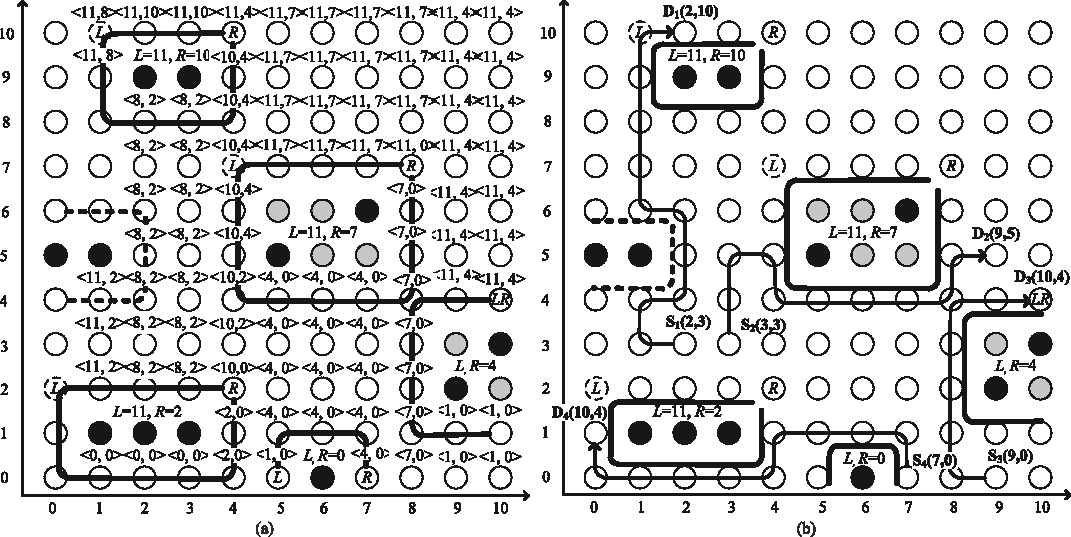
\includegraphics[width=0.95\textwidth]{ZD-fig7}
          \caption{Illustrative example. Dark, gray, and white nodes represent faulty, unsafet, and safe nodes, resp. Dashed bold lines represent $l$-chains, solid bold lines represent $f$-chains. The 2-tuple <$c$, $f$> indicates the value of \textit{ceiling} and \textit{floor} registers. Nodes without labeled values have the unchanged initialized value <11, 0>. (a) Network status. (b) Routing example.}
        \label{fig:ZD-fig7}
\end{figure}


Nodes above and below some kinds of faulty blocks should update their \textit{floor} and \textit{ceiling} registers, resp. For example, node (6, 7) will set its floor register to 7 when it finds that it is on the north boundary of an FB-5 faulty block. The position of faulty blocks is distributed inside each column. We could find that node (6, 1) does not update its \textit{floor} register because we do not care about the position of faulty blocks touching north or south network edges.

Figure \ref{fig:ZD-fig7}(b) shows four routing examples using the ZoneDefense routing. When we talk about the ceiling, floor, and two reference nodes, please refer to Figure \ref{ZD-fig7}(a) for their values.

The first packet, $S_{1}(2, 3) \rightarrow D_{1}(2, 10)$, is routed to west by the Default-Routing because the destination is higher than the \textit{ceiling}. The packet is further routed north to node (1, 4), where the LChain-Routing will be used. Since the current node is on the south block boundary and the destination is higher than the current node, the packet is routed east to corner (2, 4). Then, the packet is routed to north as the Default-Routing returns “west” and the destination is higher than the current node. At the northeast corner, the LChain-Routing agree with the Default-Routing because the northeast corner only cares about the packet whose destination is lower than itself. When the packet arrives at node (1, 6), it is routed to north because the destination is on the northeast to the current node. When the packet arrives at node (1, 8), the FChain-Routing will be used. The southwest corner of $f$-chain only cares about the packet whose destination is lower than the right reference node. Thus, the packet is routed to north according to the Default-Routing. At node (1, 9), which is on the west block boundary, the packet is routed to north as the destination is higher than the right reference node. Until reaching the northwest corner, the packet is routed east to the destination. The routing paths of other packets are also shown in Figure \ref{fig:ZD-fig7}(b), but we omit the detailed description due to the limited space of this paper.

\subsection{Proof of Fault-Tolerant Routing}
Dally and Seitz \cite{dally1988deadlock} have proved that a network is deadlock free if the corresponding channel dependence graph (CDG) is acyclic. Later, Chiu \cite{chiu2000odd} has proved that an CDG is acyclic if all rightmost columns are broken in clockwise and counterclockwise abstract cycles. Therefore, to prove the proposed ZoneDefense routing deadlock free, we will prove the corresponding CDG acyclic by showing that:

\begin{enumerate}[1)]
    \item If faults do not appear on the left network edge, no
        rightmost column can be formed;

    \item The rightmost columns introduced to tolerate faults on
        the left network edge do not form cycles.
\end{enumerate}

\textit{Lemma 1:} ES turn only appears at the west boundary of FB-2 and FB-5 faulty blocks, as well as the northeast corners of the FB-4, FB-7, and FB-8 faulty blocks.

\textit{Proof:} Assuming that the current node is node-c and a packet is routed from its west neighbor node-w. If node-c is at the west boundary of one FB-2 or FB-5 faulty block and the destination, node-d, is on the east of node-c, then the packet should be routed to south. Thus, an ES turn is introduced. Otherwise, if node-c is at the a northeast corner of one FB-4 or FB-7 or FB-8 faulty block and node-d is on the southeast of node-c, then the packet should be routed to south. Thus, an ES turn is introduced.

Now, we prove that ES turn cannot appear at other cases. We prove this by contradiction. If node-c is not at any faulty block boundary, then node-d should be on the southeast of node-c and node-w. Since packet is routed to east instead of south at node-w, node-w should be at the north boundary of a faulty block. Thus, node-c should be at the north boundary or northeast corner of that faulty block. Contradiction arises.

Otherwise, if node-c is on a faulty block boundary but at neither west boundary of FB-2 and FB-5 faulty blocks nor the northeast corner of the FB-4, FB-7, and FB-8 faulty blocks. To make an ES turn at node-c, the west and south neighbor of node-c should be safe. Thus, node-c should at one of the following positions: west and south boundary or northwest, southwest, and southeast corner of the faulty block. However, in any above cases, the packet should be routed to south instead of east at node-w. Contradiction arises.

\textit{Lemma 2:} EN turn only appears at the west boundary of FB-8 faulty blocks, as well as the southeast corners of the FB-1, FB-2, FB-4, and FB-5 faulty blocks; SW turn only appears at the southeast corners of FB-1, FB-2, FB-4, and FB-5 faulty blocks; NW turn only appears at the northeast corners of FB-4, FB-7, and FB-8 faulty blocks.

\textit{Proof:} The proofs for EN, SW, and NW turns are similar with that for ES turn and are omitted. 

\textit{Lemma 3:} The ES turn at the west boundary of FB-2 and FB-5 faulty blocks does not belong to any clockwise rightmost column.

\textit{Proof:} According to the second floor rule, the southwest corner of FB-2 and FB-5 faulty blocks update their floor registers with their y-coordinates. Thus, the ES turn at the west boundary of FB-2 and FB-5 faulty blocks cannot connect with SW turns below the southwest corner. Furthermore, SW turn cannot appear at the west boundary of faulty blocks according to Lemma 2. Therefore, the rightmost column cannot be formed.

\textit{Lemma 4:} The ES turn at the northeast corner of FB-7 faulty block does not belong to any clockwise rightmost column.

\textit{Proof:} Since SW turn cannot appear below the northeast corner of FB-7 faulty blocks, the clockwise rightmost column cannot be formed.

\textit{Lemma 5:} The EN turn at the west boundary of FB-8 faulty block does not belong to any counter-clockwise rightmost column.

\textit{Proof:} According to the second ceiling rule, the northwest corner of the FB-8 faulty blocks update its ceiling register with its y-coordinate. Thus, the EN turn at the west boundary cannot connect with NW turns above the northwest corner. Furthermore, NW turn cannot appear at the west boundary of faulty blocks according to Lemma 2. Therefore, the counter-clockwise rightmost column cannot be formed.

\textit{Lemma 6:} The EN turn at the southeast corners of FB-1, FB-2, and FB-5 faulty blocks does not belong to any counterclockwise rightmost column.

\textit{Proof:} Nodes above the southeast corners of FB-1 and FB-2 faulty blocks do not introduce NW turns, so that the EN turn at the southeast corners of FB-1 and FB-2 faulty blocks does not belong to any counter-clockwise rightmost column. Since the northeast corner of the FB-5 faulty block sets its ceiling register with its y-coordinate according to the second ceiling rule, the EN turn at the southeast corner of the FB-5 faulty block cannot connect with other NW turns. Therefore, it does not belong to any counter-clockwise rightmost column either.

\textit{Lemma 7:} The SW turn at the southeast corners of FB-1 and FB-2 faulty blocks does not belong to any clockwise rightmost column.

\textit{Proof:} The clockwise rightmost column cannot be formed because the routers above the southeast corners of FB-1 and FB-2 faulty blocks cannot introduce ES turns.

\textit{Lemma 8:} The SW turn at the southeast corner of FB-5 faulty blocks does not belong to any clockwise rightmost column.

\textit{Proof:} We prove this by contradiction. If a clockwise rightmost column is formed, there should be an ES turn above the southeast corner as well as it is connected with the SW turn. Since the northeast corner of FB-5 faulty blocks forbids the ES turn, this ES turn should be above the northeast corner. However, the northeast corner of FB-5 faulty blocks will cut off the connection between ES and SW turns because it sets floor register with its y-coordinate. Therefore, the SW turn at the southeast corner of FB-5 faulty blocks does not introduce rightmost columns.

\textit{Lemma 9:} The NW turn at the northeast corners of FB-7 and FB-8 faulty blocks does not belong to any counterclockwise rightmost column.

\textit{Proof:} The counter-clockwise rightmost column cannot be formed because the routers below the northeast corners of FB-7 and FB-8 faulty blocks cannot introduce EN turns. 

\textit{Lemma 10:} Clockwise rightmost column can be formed if and only if the ES and SW turns appear at the northeast and southeast corners of FB-4 faulty blocks, resp.

\textit{Proof:} According to Lemmas 1 and 2, the ES and SW turns can appear at the northeast and southeast corners of the FB-4 faulty block, resp. Thus, the clockwise rightmost column can be formed with them.

Assuming a clockwise rightmost column is formed. According to Lemmas 3 and 4, the ES turn should be at the northeast corner of an FB-4 faulty block. According to Lemmas 7 and 8, the SW turn should be at the southeast corner of an FB-4 faulty block.

\textit{Lemma 11:} Counter-clockwise rightmost column can be formed if and only if the EN and NW turns appear at the southeast and northeast corners of FB-4 faulty blocks, resp. Proof: According to Lemma 2, EN and NW turns can appear at the southeast and northeast corners of an FB-4 faulty block. Thus, the counter-clockwise rightmost column can be formed.

Assuming a counter-clockwise rightmost column is formed. According to Lemmas 5 and 6, the EN turn should be at the southeast corner of an FB-4 faulty block. According to Lemma 9, the NW turn should be at the northeast of an FB-4 faulty block.

\textit{Lemma 12:} Rightmost columns on the boundary of FB-4 faulty blocks cannot form cycles.

\textit{Proof:} According to Lemmas 10 and 11, the rightmost columns always stick to the boundary of FB-4 faulty blocks. Furthermore, 180-degree turns are not allowed. Thus, cycles cannot be formed because there are no corresponding leftmost columns since FB-4 faulty blocks touch the left network edge.

\textit{Theorem 13:} ZoneDefense routing is deadlock free. 

\textit{Proof:}

\begin{enumerate}[1)]
    \item If the network is fault free, the ZoneDefense routing only allows the WN, WS, NE, and SE turns. Thus, the CDG is acyclic.
    \item Otherwise, if the network has faults: 
        \begin{enumerate}[a)]
            \item If none of the faults locate on the left network edge, no rightmost columns can be formed according to Lemmas 10 and 11. Thus, the CDG is still acyclic.
            \item Otherwise, if some faults locate on the left network edge, the rightmost columns, which are introduced to tolerate faults on the left network edge, never form cycles according to Lemma 12. Thus, the CDG is still acyclic.
        \end{enumerate}
\end{enumerate}

To sum up, wherever the faults locate, the ZoneDefense routing is deadlock free according to Dally and Seitz’s theory \cite{dally1988deadlock} since the CDG is always acyclic. With a nonminimal routing, packets may encounter livelock and move through the network without ever reaching their destination. In the following, we prove that the proposed ZoneDefense routing is livelock free.

\textit{Theorem 14:} ZoneDefense routing is livelock free.

\textit{Proof:} In the absence of faults, ZoneDefense routing is minimal, and is thus livelock free. In the presence of faults, the ZoneDefense is minimal if the source and destination are not blocked by faults, and is thus livelock free. If they are blocked by faults, packets may be misrouted west or along the fault chains. Misrouting packets to west will be ended, if any one of the three conditions holds: 1) the destination is higher than current node and is lower than the ceiling, 2) the router is lower than current node and is higher than floor, or 3) the router is on the left network edge. Obviously, after misrouting west for finite hops, one of the three conditions will definitely holds true and terminates the misrouting phase. Misrouting along the fault chain will be ended, if the current router and the destination are on the same side of the faulty block. Furthermore, each faulty block introduces at most two (one for each kind) misrouting phases to a packet, and a packet encounters each faulty block at most once. Therefore, the packet will definitely reaches its destination after finite misrouting phases introduced by a finite number of faulty blocks. The network is thus livelock free.


\subsection{Experiment Result Analysis}
This section will compare the ZoneDefense routing with previous work proposed in the literatures \cite{wu2003fault} \cite{zhang2008reconfigurable}. We select them  as the baseline routing algorithms because they do not use virtual channels. Literature \cite{glass1993fault} is not compared since it only tolerates one fault. Literatures \cite{fu2011new} \cite{mejia2006segment} \cite{rodrigo2010addressing} are not compared because they require off-line analysis. Literatures \cite{fick2009highly} \cite{fick2009vicis} are not compared since they use routing tables that cannot be compressed according to their routing algorithms.

\subsubsection{Fault Model Comparison}
The fault model is important since it determines the percentage of supported fault distributions, the number of sacrificed fault-free nodes, and the reconfiguration time (i.e., the time for a network to be stable after the detection of a fault). The proposed ZoneDefense routing adopts the defense zones to include faults, literature \cite{wu2003fault} utilizes multiple convex faulty blocks, and literature \cite{zhang2008reconfigurable} utilizes only one convex faulty block. As for \cite{wu2003fault}, if faults appear at network edges or the columns adjacent to left and right network edges, all nodes of corresponding network edges or columns will be disabled.

These simulations are first carried out in an $8 \times 8$ mesh, and then in a $16 \times 16$ mesh to show the scalability. The network is assumed to have at most 10\% faulty nodes. According to \cite{meyer1989modeling}, faulty nodes tend to be clustered instead of uniformly distributed. To generate clustered faults, we randomly select the first faulty node, and select the sequencing faulty nodes with extra 10\% possibility to neighbors of previously selected faulty nodes. For the 8 × 8 mesh with one and two faults, there are 64 and 2016 different fault distributions, resp. In such cases, all fault distributions are simulated. If more than two faults are assumed, we randomly select 10 000 different fault distributions to save simulation time. For the $16 \times 16$ mesh, on the other hand, we only exhaust the 256 different one-fault distributions. If more than one fault is assumed, we also simulate 10 000 randomly selected fault distributions.

1)\textit{Coverage of Fault Distributions:} We first report the coverage of fault distributions of simulated fault-tolerant routing algorithms. Specifically, if the formed faulty blocks divide the network into several unconnected parts, we say that the fault distribution is not supported by the ZoneDefense routing and the routing algorithm proposed in \cite{zhang2008reconfigurable}. According to \cite{wu2003fault}, network cannot be partitioned since faulty or unsafe nodes never locate on the new reconfigured network edges. However, all fault-free nodes may be disabled in worst cases. In such cases, we say that the fault distribution is not supported by the routing algorithm proposed in \cite{wu2003fault}.

The simulation results are shown in Figure \ref{fig:ZD-fig8}, where the x-axis represents the number of faults inserted into the network, the y-axis indicates the percentage of supported fault distributions. Particularly, “Wu \cite{wu2003fault}” represents the routing algorithm proposed in \cite{wu2003fault}, “Zhang \cite{zhang2008reconfigurable}” represents that proposed in \cite{zhang2008reconfigurable}, and “Proposed” represents the proposed ZoneDefense routing.

\begin{figure}[h]
    \centering
        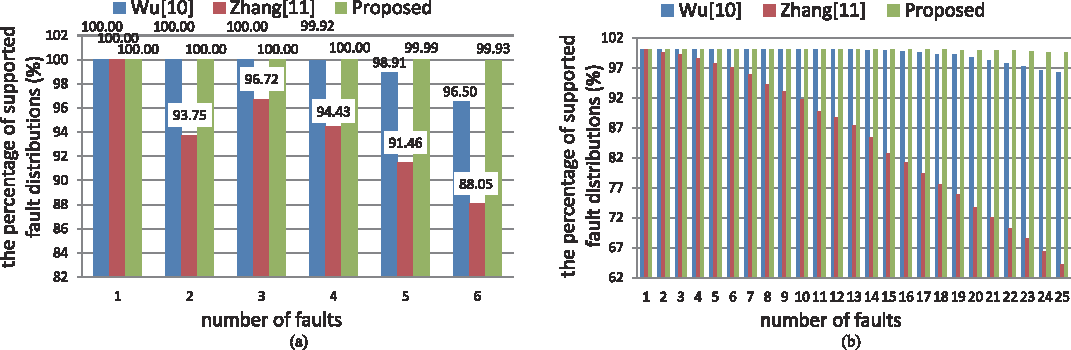
\includegraphics[width=0.95\textwidth]{ZD-fig8}
          \caption{Coverage of fault distributions. (a)$8 \times 8$ mesh. (b)$16 \times 16$ mesh.}
        \label{fig:ZD-fig8}
\end{figure}

In the $8 \times 8$ mesh [see Figure \ref{fig:ZD-fig8}(a)], all routing algorithms can tolerate all one-fault distributions. If two or three faults are inserted, the ZoneDefense routing and \cite{wu2003fault} also can tolerate all distributions. However, \cite{zhang2008reconfigurable} only tolerates 93.75 and 96.72\% distributions, resp. In three-faults case,  \cite{zhang2008reconfigurable} got better result than that in two-faults case because 1) only 10 000 fault distributions are simulated in threefaults case, and 2) clustered faults are assumed. Actually, if all three-fault distributions are simulated, the results should be worse than that in two-faults case. As the number of faults increases, the percentage of supported fault distribution degrades for all routing algorithms. However, for the ZoneDefense routing, the degradation is negligible. For example, even with six faults, 99.93\% fault distributions still can be tolerated. For \cite{wu2003fault}, the degradation is moderate. For example, 96.5\% distributions still can be tolerated with six faults. On the other hand, for \cite{zhang2008reconfigurable}[11], the degradation is significant. For example, only 88.05\% of the six-faults distributions can be tolerated.

When the network size increases, the relative performance of these algorithms do not change [see Figure \ref{fig:ZD-fig8}(b)]. However, the difference between \cite{zhang2008reconfigurable} and other two algorithms becomes much larger. For example, only about 65\% of the 25-faults distributions can be tolerated by \cite{zhang2008reconfigurable}, but more than 97\% and 99\% distributions can be tolerated by \cite{wu2003fault} and the ZoneDefense routing, resp.

According to the above analysis, ZoneDefense routing and \cite{wu2003fault} get much better results than \cite{zhang2008reconfigurable}. In the next simulation, we will find that although \cite{wu2003fault} can support most of the fault distributions as the ZoneDefense routing, \cite{wu2003fault} will sacrifice much more fault-free nodes.

2)\textit{Number of Sacrificed Nodes:} To avoid deadlock, some fault-free nodes should be sacrificed. They may be included into faulty blocks or explicitly disabled, and are not allowed to send and receive packets. Thus, the associated core and caches also cannot be utilized by applications. This section will compare the number of nodes sacrificed by the ZoneDefense routing and previous work \cite{wu2003fault}, \cite{zhang2008reconfigurable}.

The simulation setup is same with the simulation discussed in above section, and the results are shown in Figure \ref{fig:ZD-fig9}. For one fault in an $8 \times 8$ meshes [see Figure \ref{fig:ZD-fig9}(a)], the ZoneDefense routing and \cite{zhang2008reconfigurable} do not sacrifice fault-free nodes. However, \cite{wu2003fault} will sacrifice 7.4 fault-free nodes in average. Because if the fault appears at network edges or the columns adjacent to left and right network edges, all nodes of the edge or column will be disabled. When the number of faults increases, the number of nodes sacrificed by \cite{wu2003fault}, \cite{zhang2008reconfigurable} significantly increases. For example, when six faults are assumed, \cite{wu2003fault} and \cite{zhang2008reconfigurable} sacrifice 27.3 and 16.5 fault-free nodes in average, resp. On the other hand, the ZoneDefense routing only sacrifices 3.7 nodes in average. The number of \cite{zhang2008reconfigurable} gets better results in three-faults case than in two-faults case due to the two same reasons discussed in above section.

\begin{figure}[h]
    \centering
        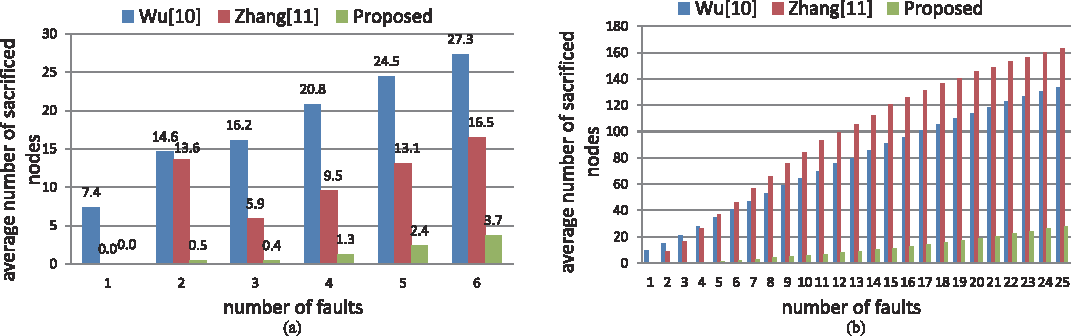
\includegraphics[width=0.95\textwidth]{ZD-fig9}
          \caption{Average number of sacrificed nodes. (a)$8 \times 8$ mesh. (b)$16 \times 16$ mesh.}
        \label{fig:ZD-fig9}
\end{figure}

When the network size increases, the absolute number of nodes sacrificed by all routing algorithms is increased as the average distance between faults increases. The ZoneDefense routing also gets better results than its two counterparts. For example, if 25 faults are assumed, the ZoneDefense routing sacrifices about 28 fault-free nodes. On the other hand, \cite{wu2003fault} and \cite{zhang2008reconfigurable} sacrifice about 133 and 163 fault-free nodes, resp. The difference is huge. If fewer than five faults are assumed, \cite{zhang2008reconfigurable} gets better results than \cite{wu2003fault}. Otherwise, \cite{zhang2008reconfigurable} sacrifices more because a big-size faulty block is usually formed with the large number of faulty nodes.

According to the above two simulations, we could find that the ZoneDefense routing can support most fault distributions with a small number of sacrificed nodes. Although \cite{wu2003fault} also can support most fault distributions, the number of sacrificed fault-free nodes is huge. As for \cite{zhang2008reconfigurable}, large fractions of fault distributions cannot be tolerated as well as a large number of nodes are sacrificed.

3)\textit{Reconfiguration Time:} The reconfiguration time or the convergence time is the time for the network to be stable after the faults are detected. In this simulation, we assume a static reconfiguration algorithm, such as the one proposed in \cite{rodeheffer1991automatic}, and omit the time for draining old packets by assuming that the network is empty when faults are detected.

The simulation setup is same with above two simulations, and the results are shown in Figure \ref{fig:ZD-fig10}. For $8 \times 8$ meshes [see Figure \ref{fig:ZD-fig10}(a)], these three routing algorithms get similar results. The ZoneDefense routing takes a longer time to be stable than \cite{wu2003fault} as it needs to spread faulty blocks’ information in corresponding columns. The reason why \cite{zhang2008reconfigurable} requires the longest time to be stable is that each node should check whether there is faulty or unsafe node in its row and column.

In $16 \times 16$ meshes [see Figure \ref{fig:ZD-fig10}(b)], the reconfiguration time increases as expected. \cite{zhang2008reconfigurable} also takes the longest time to be stable. The ZoneDefense routing takes a longer time than \cite{wu2003fault} if the number of faults is smaller than nine because ZoneDefense routing should spread faulty blocks’ information in corresponding columns. Otherwise, \cite{wu2003fault} takes a longer time because the possibility of disabling a network edge or column increases.

\begin{figure}[h]
    \centering
        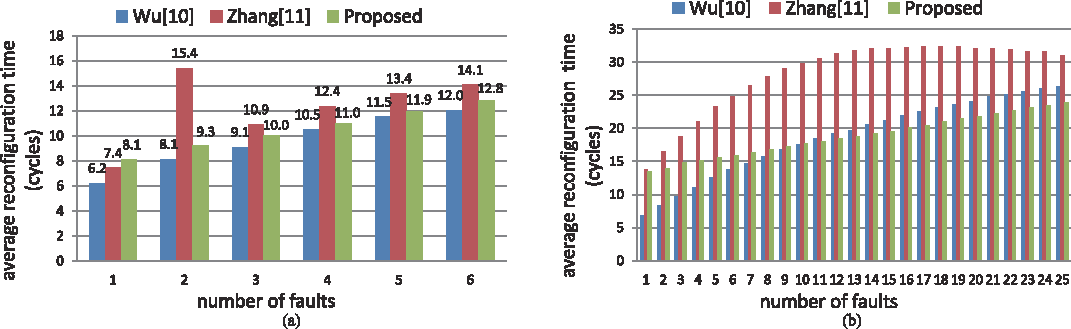
\includegraphics[width=0.95\textwidth]{ZD-fig10}
          \caption{Average reconfiguration time. (a)$8 \times 8$ mesh. (b)$16 \times 16$ mesh.}
        \label{fig:ZD-fig10}
\end{figure}

\subsubsection{Performance Analysis}
In this simulation, we utilize a cycle-accurate NoC simulator, the BookSim \cite{dally2004principles}, to carry out the simulations. BookSim provides a flexible way to configure NoC parameters, such as network topology and routing algorithm. By maintaining a global clock, BookSim could keep the simulation cycleaccurate. In the following simulations, router pipeline depth is assumed as four and link traversal latency is one. The round-robin policy is adopted to select requesting inputs in switch allocation stage. Although we assume a canonical router architecture instead of the aggressive state-of-the-art ones, such as lookahead routing and speculation, it is fair for evaluating fault-tolerant routing algorithms. For each routing algorithm, we assume that there is one virtual channel per physical channel, and each virtual channel contains an FIFO with eight entries to hide the round-trip latency of flow-control credits.

In this simulation, we first assume the network topology is $8 \times 8$, and simulate the cases with one, three, and five faults. For the one-fault case, we simulate all 64 fault distributions and report the average results. For three-faults and fivefaults cases, we simulate 100 randomly selected different fault distributions to save simulation time. To show the scalability of routing algorithms, we further do simulations in $16 \times 16$ meshes with one, eleven, and twenty one faults. For each case, we simulate 100 randomly selected different fault distributions to save simulation time.

Under uniform traffic pattern, a safe node can send packets to all other safe nodes with the same possibility. The simulation results are shown in Figure \ref{fig:ZD-fig11}, where the x-axis represents the injected traffic load, i.e., the number of flits injected to the network per cycle, and the y-axis shows the average packet latency.

In $8 \times 8$ meshes [see Figure \ref{fig:ZD-fig11}(a)], these three routing algorithms get similar performance. For example, all of them will be saturated if more than six flits are injected per cycle for one-fault case. The main reason is that the average packet latency is largely determined by the worst case performance, which often happens when the faults locating in the center of the network. Furthermore, the main difference between ZoneDefense routing and its two counterparts \cite{wu2003fault}, \cite{zhang2008reconfigurable} is the way they treat the faults on network edges. Therefore, they will get similar worst case performance. The packet latency in worst case is often much larger than that in other cases, so that the average packet latency is similar for these three routing algorithms.

\begin{figure}[h]
    \centering
        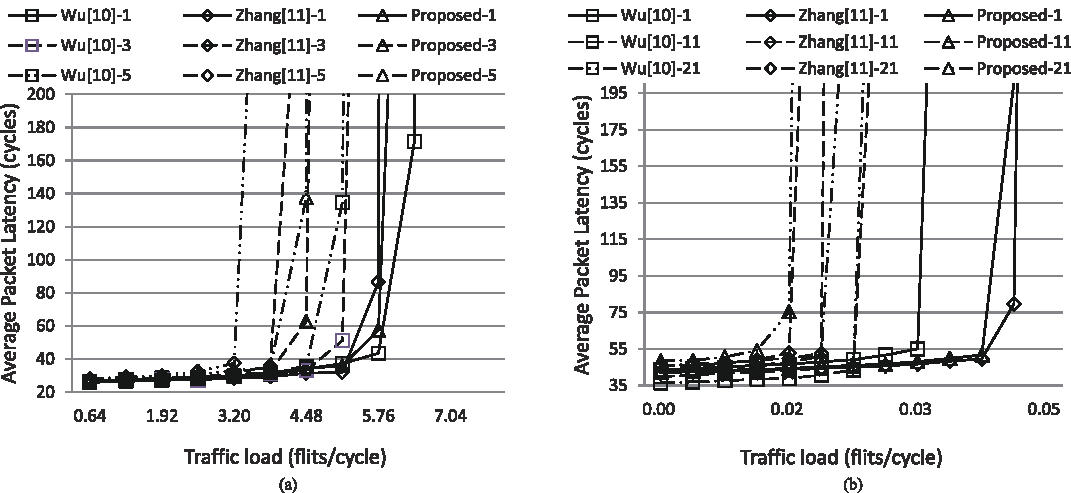
\includegraphics[width=0.95\textwidth]{ZD-fig11}
          \caption{Average packet latency under uniform traffic pattern. (a)$8 \times 8$ mesh. (b)$16 \times 16$ mesh.}
        \label{fig:ZD-fig11}
\end{figure}

As the number of faults increases, the network performance degrades. For example, the network will be saturated if more than five flits are injected per cycle for three-faults case. For \cite{wu2003fault} and the ZoneDefense routing, more faults usually translate into more faulty blocks or defense zones. Thus, the possibility of congestion increases as the congestion often happens at the boundaries of faulty blocks and defense zones. For \cite{zhang2008reconfigurable}, more faults often translate into a bigger faulty block. Since the boundary of the faulty block gets longer, the possibility of congestion increases. Furthermore, as shown in Figure \ref{fig:ZD-fig9}, the number of sacrificed nodes increases as the number of faults increases. Thus, the number of left fault-free nodes is reduced, so that the congestion problem aggregates as the injection rate per node increases. If the number of faults increases further, the network performance does not degrade notably. For example, as for the ZoneDefense routing and \cite{wu2003fault}, they get similar performance in three-faults and five-faults cases. \cite{zhang2008reconfigurable} gets moderate performance degradation when the number of faults increases from three to five. The main reason is also that the worst case fault distribution determines the average network performance.

In $16 \times 16$ meshes [see Figure \ref{fig:ZD-fig11}(b)], the ZoneDefense routing and \cite{zhang2008reconfigurable} get similar network performance, which
is much better than \cite{wu2003fault} in one-fault case. The reason is that \cite{wu2003fault} sacrifices about ten fault-free nodes in average as shown in Figure \ref{fig:ZD-fig9}(b), so that the injection rate per node for \cite{wu2003fault} will be larger than other two algorithms. Therefore, \cite{wu2003fault} get saturated earlier than others. As the number of faults increases, \cite{zhang2008reconfigurable} sacrifices more nodes than \cite{wu2003fault}. Therefore, \cite{wu2003fault} gets better performance than \cite{zhang2008reconfigurable} as its injection rate per node is relatively low. As for the ZoneDefense routing, its performance is little lower than its two counterparts. The reason is that the ZoneDefense routing sacrifices much fewer nodes than \cite{wu2003fault}, \cite{zhang2008reconfigurable} by forming many small defense zones. As the number of defense zones increases, the possibility of congestion increases.

According to above simulations, we could find that the ZoneDefense routing could get similar network performance as its counterparts in $8 \times 8$ meshes regardless of the number of faults. When the network size increases, such as in $16 \times 16$ meshes, the ZoneDefense routing and \cite{zhang2008reconfigurable} get better results than \cite{wu2003fault} at first. As the number of faults increases, the network performance of ZoneDefense routing degrades a little more than its counterparts. However, compared with \cite{wu2003fault}, \cite{zhang2008reconfigurable}, the degradation of network performance is moderate.

\subsubsection{Overhead Analysis}
In the following of this section, we will analyze the area and timing overhead of the proposed ZoneDefense routing. The routers are assumed to have five input and output ports. Five virtual channels per physical channel are utilized to realize five virtual networks. Each virtual channel has eight buffers to temporally store flits whose size is assumed as 64-bits. The round-robin arbiter proposed in the literature \cite{shin2002round} is used to implement virtual-channel and switch allocators. Note that we extend \cite{zhang2008reconfigurable} to tolerate one faulty block. To this end, \cite{zhang2008reconfigurable} adopts the same chain rules as the ZoneDefense routing. The main differences between \cite{zhang2008reconfigurable}-extended and the ZoneDefense routing are that 1) the “default routing” of \cite{zhang2008reconfigurable} is the $X-Y$ routing, and 2) fault chains do not share boundaries in \cite{zhang2008reconfigurable}.

The router area, which is normalized to the number of two-input NAND gates, is shown in the first row of Table \ref{tab:area-eval}. According to the simulation results, the area overhead of the ZoneDefense routing compared with \cite{wu2003fault} and \cite{zhang2008reconfigurable} (2.6 and 1.1\%, resp.) is very small. According to the results reported by Intel in the literature \cite{vangal200880}, each router occupies about 11\% of the tile area. Thus, the area overhead per tile (0.3 and 0.1\%, resp.) is negligible as shown in the second row of Table \ref{tab:area-eval}.

\begin{table}[h]
    \caption{Area Evaluation (Two-Input NAND Gates)}
    \begin{tabular}{|c|c|c|c|} 
        \hline
        & Wu \cite{wu2003fault}  & Zhang \cite{zhang2008reconfigurable} & Proposed Design Compared with Wu \cite{wu2003fault} and Zhang \cite{zhang2008reconfigurable} \\ \hline
                    Router Area & 19048  & 19336    & 19541(2.6\%, 1.1\%)   \\ \hline
                    Tile Area   & 173165 & 175788   & 177651 (0.3\%, 0.1\%) \\ \hline                         
    \end{tabular}
    \label{tab:area-eval}
\end{table}

The reconfiguration operations, such as forming defense zones in the ZoneDefense routing and forming faulty blocks in \cite{wu2003fault} and \cite{zhang2008reconfigurable}, do not add delay to the critical path of routers. Therefore, we only compare the routing delay of these three routing algorithms. The virtual-channel allocation stage is the critical stage of routers in our simulations. If the routing delay of \cite{wu2003fault}, \cite{zhang2008reconfigurable} (extended), and the ZoneDefense routing are normalized to the delay of the critical stage, the results are 0.83, 0.8, and 0.96, resp. Therefore, the ZoneDefense routing does not introduce timing overhead since the critical stage does not change.

\subsection{Discussion}
Based on the defense zone fault model, this paper proposed the ZoneDefense routing to reduce the large number of fault-free nodes sacrificed by state-of-the-art fault-tolerant routing algorithms. The ZoneDefense routing was theoretically proved to be deadlock and livelock free. With it, packets could find the faulty blocks in advance and route around them without introducing unexpected turns. Since the complexity of avoiding deadlock was reduced, the unexpected operations, such as including all faults into one faulty block or disabling all nodes of faulty network edges and columns, can be avoided. Extensive simulations showed that the number of sacrificed fault-free nodes is significantly reduced as well as the coverage of fault distributions and reconfiguration time is improved. Furthermore, the ZoneDefense routing does not degrade the network performance in the absence of faults and could get similar network performance as the previous work with negligible overhead. Taking all factors into consideration, we believed that the ZoneDefense routing is better than state-of-the-art fault-tolerant routing algorithms designed for NoCs without virtual channels.

\section{NoC Fault Tolerance with Data Path Salvaging}

\subsection{Fault-tolerant Router Architecture Overview}
In the proposed RevivePath scheme, different techniques are applied to protect the on-chip router data path and control path respectively. The control path including routing computing logic, virtual channel allocator, and switch allocator are critical to NoC normal operation but it usually consumes only minor chip area. Therefore, direct redundancy strategy is applied in RevivePath. For the data path, we takes advantage of the inherent regular structure and exploits the redundancy within these structures to salavge the data path of NoCs.

\begin{figure}[h]
      \centering
        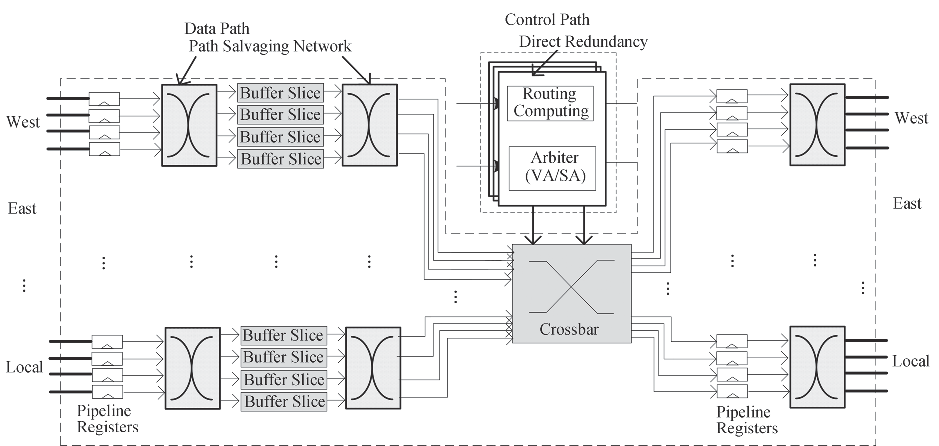
\includegraphics[width=12cm]{DPS-fig3}
        \caption{General Architecture of RevivePath.}
        \label{fig:dps-fig3}
\end{figure}


Figure \ref{fig:dps-fig3} shows the general architecture of RevivePath. In this example, links, buffers and the crossbar are partitioned into four slices. Behind links, buffers and the crossbar network, the path salvaging networks are inserted to salvage the left slices when encountering faults. Since the direct redundancy in control path is a mature idea, this subsection will mainly introduce the technique used in the data path. Data path is regular and can be regarded as many independent, identical parallel slices. A 64-bit link can be seen as four 16-bit link slices; a 64-bit FIFO can be viewed as four 16-bit FIFO slices; a 64-bit Mux which constructs the crossbar can also be divided into four 16-bit Mux slices. Whenever partial slices fail, the remaining slices can be reused to continue transmitting data in TDM mode. Data path salvaging organizes the data path components as a group of workable subcomponents, which backup each other. Details for the scheme will be explained in the following subsections.

\begin{figure}[h]
      \centering
        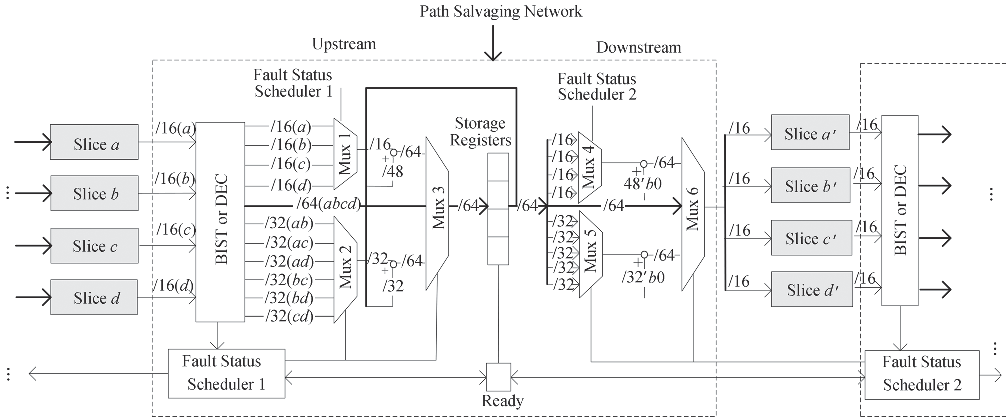
\includegraphics[width=12cm]{DPS-fig4}
        \caption{Data Path Salvaging Structure.}
        \label{fig:dps-fig4}
\end{figure}


Figure \ref{fig:dps-fig4} shows the detailed structure of data path salvaging. Data slices in this figure indicate data path components both in the downstream and upstream of links, crossbar or pipeline register. When some of the upstream data slices fail, the built-in self-test technique \cite{fick2009highly} \cite{alaghi2007online} or detection error codes (DEC) can be employed in the o®-line or on-line environments to detect the failures. The faulty information of the slices is then recorded in the registers of the fault status scheduler.

The upstream fault status scheduler is initialized by the upstream fault status registers after detecting error, and recon¯gures the path salvaging network between storage registers (in the middle of Figure \ref{fig:dps-fig4}) and upstream data slices cycle by cycle to reconstruct an integrated data in storage registers using data fragments. Similarly, the downstream fault status scheduler keeps the storage registers and downstream data slices matched. The ready °ag is a sign indicating whether data in storage registers is available. When it is set invalid, all the logic driven by storage registers has to be stalled. When it is set valid, the downstream fault status scheduler will get to work. However, if the storage register fails, the whole structure corrupts. In addition, when data slices in this figure are actually buffers, there is probably no explicit storage registers as depicted. To address the corner situations, we remove a data slot from each buffer to serve as a storage register. With simple bypass design, the special storage registers will not introduce additional pipeline latency. 

\subsection{Fault-tolerant Router Implementation}
Figure \ref{fig:dps-fig4} exhibits the slices salvaging hardware structure. It mainly consists of fault detection circuits (BIST or detection error circuits), fault status schedulers, networks constructed by MUXs, to together transfer available upstream data slices to next links. This process can be divided into two parts: upstream data to storage registers, and storage registers to downstream. Available upstream data slices are selected according to upstream fault status. Data path in the example is split into four slices. Since the situation with three slices available in upstream data slices is simply treated as that with two to alleviate the logic design complexity, there are only three possible data width situations: single fault-free data slice, two fault-free data slices, and four fault-free data slices. Mux 1 and Mux 2 in the figure are used to extract a single valid data slice and two valid data slices respectively from the upstream data path. When all the four data slices are functional, i.e., there are no faults in the upstream data path, the data from upstream data path can then be directly stored in the storage registers. 

Data in storage registers combined with the slices chosen in the first step reconstructs 64-bit data, which corresponds to the situations with different number of fault slices, through Mux 3. Blocks in the downstream including Mux 4, MUX 5, and Mux 6, the downstream fault status scheduler are responsible for the transmission from storage registers to downstream data path. When slices of the data path in downstream fail, data connected with them are simply set to 0. Apart from the difference mentioned, the blocks in both the upstream and downstream of the data path function are running in almost the same way which will not be explained in case of repetition.

In addition, we can see from Figure \ref{fig:dps-fig4} that the slice reuse logic also has inherent fault tolerance. Mux 1, Mux 3 constitute a fault-tolerant data path when there is a single input data path slice left available; Mux 2, Mux 3 construct a fault-tolerant data path when there are two available input data path slices. Furthermore, when there are no faults at all, Mux 3 sustains fully functional data path. As fault-tolerant data paths are closely coupled with speci¯c available data path slices, the probability that specific fault-tolerant data path fails and corresponding slice fault status occurs at the same time is quite low. Consequently, the slice reuse structure is quite resilient, especially compared with conventional design such as redundancy.

Take a specific setup as an example. If slice a is faulty, the BIST or DEC will detect this fault and send a fault vector [0111] to fault status scheduler 1. There is only one faulty slice, so it will be simply treated as two fault-free slices situation. Therefore, the path /32(cd) is selected. The transmissions are duplicated through the path /32(cd), Mux 3 and then 64 bits will be stored in storage registers. The ready flag is set valid until all 64 bits are reconstructed.

\begin{figure}[h]
      \centering
        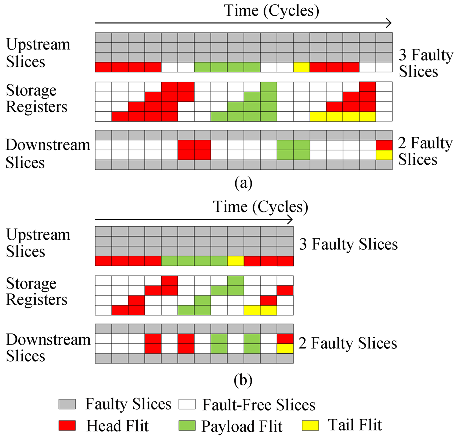
\includegraphics[width=8cm]{DPS-fig5}
        \caption{Temporal-spacial distribution example of pipeline and intermittent style under different fault configurations. (a) Intermittent style. (b) Pipeline style}
        \label{fig:dps-fig5}
\end{figure}


When some faulty slices are found, upstream data path has to wait for an assembled data in the storage register until the ready °ag is set valid. At the same time, downstream data path must also pend for fully free storage registers when the ready flag is set invalid. We denote this transmission style as "Intermittent Transmission". The temporal-spacial distribution example of intermittent style is shown in Figure \ref{fig:dps-fig5}(a). There are three faulty slices in upstream. Therefore, it takes 4 cycles to assemble the total data in storage registers. After this, the data will be transported to downstream in two cycles since there are two faulty slices in downstream. We can see that it takes the intermittent transmission style 18 cycles to complete the packet transmission including head flits, body flits and tail flit. This style is not e±cient since the downstream has to wait for the upstream data.

In order to address this less e±cient problem, we propose a new transmission style: pipeline transmission style. Compared with intermittent transmission, as long as there are available data slices in storage registers, they can be accessed and sent to the next pipeline. The stalling time is reduced. In the same faulty situ
ation as Figure \ref{fig:dps-fig5}(b), the pipeline transmission style costs only 12 cycles. Apparently, the pipeline transmission style outperforms the intermittent transmission style.

However, one thing should be noted that, when an integrated data is necessary for downstream data path such as routing computing, the intermittent transmission style will remain functional while slice pipeline transmission style will be powerless. Slice Fault Status Association. When slice reuse technique is applied, the fault status of neighboring data path slices influences each other. Assume that the fault-free slice number from input links of router A to buffers in router B (links, buffers, crossbar, links) are $s_1$, $s_2$, $s_3$, $s_4$ respectively. When $s_{2} \leq s_{1}$, links provides more data slices than what buffers could accommodate each cycle, thus pipeline registers between the links and buffers will be overlaid. In case of the problem, links will have to wait for the release signal of the pipeline registers. As a result, it makes the flow control more complex and inefficient. When $s_{4} \leq s_{3}$, the problem is similar. To guarantee a correct and efficient pipeline, the available slice numbers of the data path components are then modified as $v_1$, $v_2$, $v_3$, $v_4$ respectively where $v_{1} \leq v_{2}$, $v_{3} \leq v_{4}$. Since the slice reuse structure between the buffer and crossbar employs intermittent transmission style, $v_2$ is independent with $v_3$. Therefore, the data path slice status correlation is limited between buffers of neighboring routers, which will not affect the scalability of the proposed method. In addition, when the number of available data path slices cannot be fully used in TDM mode, it will then be degraded to simplify hardware design. For example, when a data path is split into four slices and three of them are fault-free, it will be degraded to 2. Accordingly, the maximum available buffer capacity will be modified to adapt the flow control usually in flit granularity.

\subsection{Experiment Result Analysis}

\subsubsection{Area Overhead}
In order to evaluate the area overhead, we synthesize the proposed router design under 200 MHz. The flit width is 64-bit, and the bu®er capacity for each input port is 8 flits. Different fault-tolerant mechanisms including redundancy, detection error code, and path salvaging network are employed in this router. To get a comprehensive perspective of slicing technique, four different path salvaging network con¯gurations: Our-4 (data path salvaging router with four slices), Our-2 (data path salvaging router with two slices), Our-M (data path salvaging router with mixed slice number), i.e., the buffer and link adopt four slices, while the crossbar chooses two slices, and Our-D (data path salvaging router discarding crossbar protection), i.e., the buffer and link are still divided into four slices while the crossbar simply goes unprotected, are synthesized under the same situation. Experimental results show that the area overhead of the four routers are 65.4\%,
26.5\%, 52.46\% and 45.9\% respectively. Without link slicing logic, the area overhead of the routers turn to be 45.9\%, 20.0\%, 33.1\% and 26.5\% respectively.

\begin{figure}[h]
      \centering
        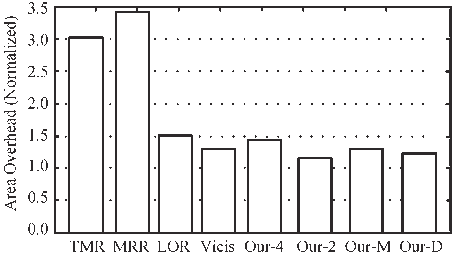
\includegraphics[width=7cm]{DPS-fig6}
        \caption{Area overhead comparison among routers with different fault-tolerant design approaches.}
        \label{fig:dps-fig6}
\end{figure}

Figure \ref{fig:dps-fig6} presents the area overhead of TMR (3-modular redundancy), MRR (most reliable router) \cite{constantinides2006bulletproof}, LOR (least overhead router)\cite{constantinides2006bulletproof}, Vicis\cite{fick2009highly} and the proposed designs. Note that Vicis has also considered the overhead of fault detection which costs additional 10\% area. To make a fair comparison, we have removed the area overhead of this part. Additionally, since TMR, MRR, LOR, Vicis only concentrate on logic part fault-tolerant, our proposed methods also do not include the area targeting the link fault tolerance. In this figure, it can be seen that TMR and MRR which employ direct replication consume more than 100\% area overhead. LOR, Vicis and the proposed design in this paper develop router's inherent redundancy with various methods, and the area overhead are mostly around 20\% to 50\%. They are more area efficient.

\subsubsection{Reliability}
The reliability also depends on the protection circuit. To evaluate reliability, Constantinides et. al. \cite{constantinides2006bulletproof} defined a new metric called SPF (Silicon Protection Factor), which is the number of faults that a router can tolerate before becoming afunctional normalized by the area overhead. In this paper, we obtain the SPF using the following procedure: a random fault injection scheme is employed based on the area of components. When a fault falls on certain router components and the fault can still be tolerated, the counter that records the total fault injection number is increased by one. Finally, when one of the components totally corrupts and thereby induces router failure, fault injection completes. With repeated fault injection of 100 000 times, the average counter value is regarded as the average number of faults that a router can tolerate. 

\begin{figure}[h]
      \centering
        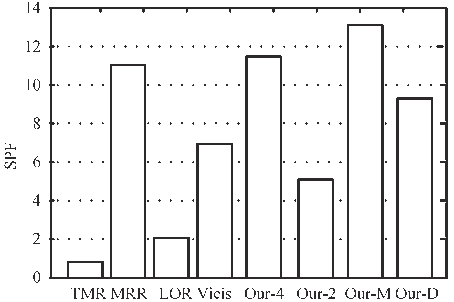
\includegraphics[width=7cm]{DPS-fig7}
        \caption{Silicon Protection Factor (SPF) Comparison of the Different Fault-Tolerant Router Design Approaches.}
        \label{fig:dps-fig7}
\end{figure}


With delicate experiments, the number of faults that Our-4, Our-2, Our-M and Our-D can tolerate is 16.80, 6.18, 17.51 and 11.84 respectively. Normalized by the area overhead, SPF of Our-4, Our-2, Our-M and Our-D is 11.52, 5.15, 13.17 and 9.36 respectively. The SPF comparison results are displayed in Figure \ref{fig:dps-fig7}. Although the SPF of MRR is also very high, the additional MRR area overhead is more than 200\%. In a complex virtual channel router, the area cost might be too large to be accepted. Vicis has a moderate area overhead and SPF. However, with similar area overhead, Our-4, Our-M and Our-D all have much higher SPF, and especially the SPF of Our-M even doubles that of Vicis. Although Our-2 has a relatively low SPF, it has the lowest area overhead. The reason that the SPF of Our-4 is lower than Our-M lies in the fact that the crossbar in planar NoC is small. So four-slice reuse method will be a little overprotected which pulls down average SPF. When the fault-tolerant method is used in a high dimension network with much larger crossbar area, Our-4 will outperform the other con¯gurations. In addition, we can also find that Our-M has higher SPF than Our-2 which indicates that the bu®er and link with four slices are more efficient than those with two slices. This is also in accordance with the experimental results shown in Figure \ref{fig:dps-fig7}.

\begin{figure}[h]
      \centering
        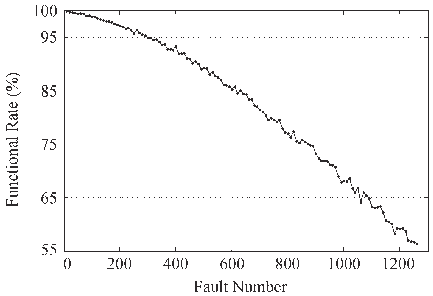
\includegraphics[width=7cm]{DPS-fig8}
        \caption{Percentage of the Available Routers in a $8 \times 8$ Torus NoC.}
        \label{fig:dps-fig8}
\end{figure}

To get an insight into the proposed method, we also evaluate the network reliability. There is no specific fault tolerance routing algorithm used in this paper, and thus we cannot make further comparison with Vicis. As torus is symmetrical and faults have equal influence on all routers, which makes the analysis scalable, we evaluate 8 £ 8 torus network reliability considering link fault as well. Any router component failure or corresponding output link failure is assumed as node failure. When additional logic used as fault tolerance fails, the protected component is assumed to be corrupted too. In this case, Figure \ref{fig:dps-fig8} shows available node number when the network suffers 0 to 1300 faults (it also equals such a fault rate per gate that scales from 0 to 1/2000). When the fault number is no more than 300, 95\% nodes keep fully functional. Even when the fault number jumps to 1000, 70\% nodes struggle to survive successfully.

\begin{figure}[h]
      \centering
        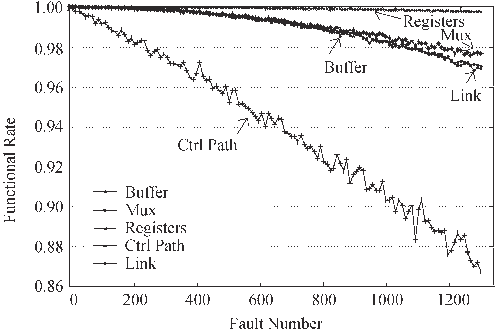
\includegraphics[width=7cm]{DPS-fig9}
        \caption{Percentage of Available NoC Components in a $8 \times 8$ Torus NoC.}
        \label{fig:dps-fig9}
\end{figure}


Most of the fault tolerance routings allow partial nodes to remain functional, so we further analyze the component status in NoC. Figure \ref{fig:dps-fig9} exhibits NoC component fault status exposed to previous fault injection. It is surprising that when the fault number comes to 500, still 95\% of the components remain functional. Even if the fault number doubles, 90\% components survive. Therefore, with typical fault-tolerant routing, there will be more available nodes left. On the other hand, we find that when the fault number is around 1 300, 96\% data path could still be functional. Unfortunately, only 86\% control logic blocks are left, which become the bottleneck of further improvement on NoC reliability. In this paper, conventional redundancy method is used to protect control logic block, nevertheless, Mux and Demux that are used for redundancy are also exposed to fault. When Mux and Demux fault probability increases faster than that of redundancy logic, there will be reliability limit for control logic block, no matter how we improve the redundancy granularity and spare number.

\begin{figure}[h]
      \centering
        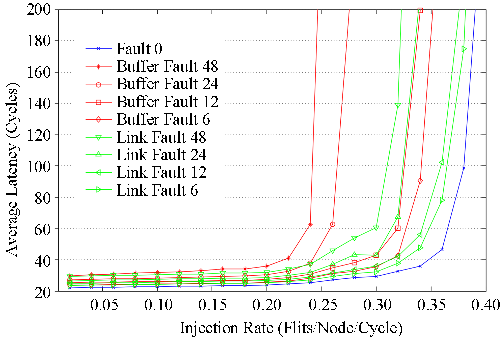
\includegraphics[width=7cm]{DPS-fig10}
        \caption{Average network latency under various fault scenarios.}
        \label{fig:dps-fig10}
\end{figure}

To evaluate the influence of the proposed data path salvaging approach on NoC performance, we implement a cycle-accurate simulator in SystemC with $4 \times 4$ 2D mesh topology constructed by wormhole routers. XY routing is employed and each input port has an 8-flit depth buffer. Each node of the network generates packets according to Poisson process. Destinations of the packets are selected randomly. 100K packets with 8 flits long per node are injected with 20K cycles warm-up before collecting performance information. We inject 6 to 48 faults on links and buffers. The simulation results shown in Figure \ref{fig:dps-fig10} illustrate that the proposed design keeps graceful performance degradation when the number of faults increases. Moreover, in the proposed design, both single-slice fault and double-slice fault are assumed to be equivalent, link faults result in associated crossbar partially working, and buffer faults lead to disabling of corresponding links and crossbar. It means that performance of 6 buffer faults equals that of 6 to 36 faults including 6 to 12 buffer faults, 0 to 12 links faults and 0 to 12 crossbar faults. Similarly, performance of 6 link faults is equivalent to that of 6 to 24 faults including 6 to 12 link faults and 0 to 12 crossbar faults. The other fault situations also implicit a much larger number of fault situations. Thus the NoC performance will keep stable in a large range of faults.

\subsection{Discussion}
In this paper, we exploited NoC inherent redundancy by splitting large NoC components of data path into slices, each of which is able to maintain the function of the whole component in presence of partial failures using TDM. For tiny logic with comparatively low fault probability, conventional redundancy or ECC is employed. Evaluation result shows that the proposed design provides several con¯gurations with high reliability and low overhead. The area overhead varies from 26.5\% to 65.4\% and SPF scales from 5.15 to 13.17. When the network suffers medium fault rate, 90\% nodes in $8 \times 8$ torus keep fully functional. Even if the network is exposed to higher fault rate, about 55\% nodes survive, and more than 86\% NoC components work well, which promises a much larger number of available nodes with conventional fault-tolerant routing. The simulation also indicates that the NoC performance degrades gracefully when fault rate rises dramatically.

\section{Summary}
To be added.

\bibliographystyle{plain}
\bibliography{refs}


